% arara: clean: {
% arara: --> extensions:
% arara: --> ['aux', 'log', 'pdf', 'toc']
% arara: --> }
% arara: lualatex: {
% arara: --> shell: yes,
% arara: --> draft: yes,
% arara: --> interaction: batchmode
% arara: --> }
%! arara: bibtex
%! arara: lualatex: {
%! arara: --> shell: yes,
%! arara: --> draft: no,
%! arara: --> interaction: batchmode
%! arara: --> }
% arara: lualatex: {
% arara: --> shell: yes,
% arara: --> draft: no,
% arara: --> interaction: batchmode
% arara: --> }
% arara: clean: {
% arara: --> extensions:
% arara: --> ['aux', 'log', 'toc']
% arara: --> }
\documentclass[
	12pt,
	oneside,
	appendixprefix=true
]{scrbook}
\usepackage[spanish]{babel}
\decimalpoint
\usepackage{diffcoeff}
\usepackage[intlimits]{mathtools}
\usepackage{amssymb}
\usepackage{amsthm}
\usepackage{graphicx}
\usepackage{minted}
\usepackage[
	citestyle=numeric,
	style=numeric,
	backend=biber,
]{biblatex}
\usepackage{hyperref}

\title{
	Una introducción acerca de los métodos de volúmenes finitos para
	una ecuación de transporte
}
\author{\scshape\name}
\date{\today}

% \addtokomafont{section}{\centering}
% \addtokomafont{subsection}{\centering}

\theoremstyle{definition}
\newtheorem{theorem}{Teorema}
\newtheorem{definition}{Definición}
\newtheorem{remark}{Observación}
\newtheorem{example}{Ejemplo}
\addbibresource{references.bib}

\providecommand{\name}{Carlos Aznarán} % Nombre
\renewcommand{\listingscaption}{Programa}
\renewcommand{\listoflistingscaption}{Lista de \listingscaption s}

\hypersetup{
	pdfencoding=auto,
	linktocpage=true,
	colorlinks=true,
	linkcolor=blue,
	urlcolor=magenta,
	pdfpagelabels,
	pdftex,
	pdfauthor={Carlos Aznarán Laos},
	pdftitle={Una introducción acerca de los métodos de volúmenes
			finitos para una ecuación de transporte},
	pdfsubject={Lecture},
	pdfkeywords={finite volume, pde, transport equation},
	pdfproducer={LuaHBTeX, Version 1.18.0 (TeX Live 2024/Arch Linux)},
	% bookmark=false
}

\clearpage
\pagestyle{empty}
\renewcommand*{\chapterpagestyle}{empty}


\begin{document}

\maketitle
\tableofcontents
\frontmatter

\section*{Agradecimientos}

Quiero agradecer a Dios por gozar de una buena salud, ayudándome a
obrar de bien, constituir una gran familia y mmis hijos por su amor
permanente y motivación para poder realizar este trabajo.
Quiero agradecer al estudiante Carlos Aznarán por su apoyo en la
elaboración de las animaciones.

\begin{flushright}
  \name \\
  Lima, 2 de enero de 2025.
\end{flushright}

\mainmatter

\chapter*{Introducción}

En el presente trabajo su estudio principal es de los métodos de
volúmenes finitos para la resolución numérica de problemas
hiperbólicos.
Se toma en cuenta las ecuaciones en derivadas parciales para las
leyes de conservación en el caso de problemas unidimensionales y
lineales.
Dichas ecuaciones nos permiten describir fenómenos de propagación de
ondas así como de transporte, presentes en diversas disciplinas
científicas.
Más adelante, realizamos un estudio del método de volúmenes finitos
enfocándonos en los métodos de un paso para la ecuación de
transporte, analizando la convergencia de dichos métodos.
Finalmente concluimos con una serie de simulaciones numéricas, ya que
nuestro objetivo es comprobar lo experimental con la parte teórica.
\chapter{Fundamentos básicos}\label{ch:fundaments}

Presentamos la ley de conservación lineal escalar unidimensional.
Se definen la solución asociada a un problema de Cauchy, que será
empleado para medir el error de las soluciones aproximadas.
Como problema modelo, se considera la ecuación de transporte escalar.

\section{Ley de conservación}

\begin{definition}
  Sean
  \begin{math}
    \Omega\subset
    \mathbb{R}
  \end{math}
  y
  \begin{math}
    f\colon\Omega\to
    \mathbb{R}
  \end{math}
  una función de clase
  \begin{math}
    C^{1}
    \left(\Omega\right)
  \end{math}.
  Una \textbf{ley de conservación unidimensional} es

  \begin{equation}\label{eq:differentialconservationlaw}
    u_{t}
    \left(x,t\right)+
    f_{x}
    \left(
    u\left(x,t\right)
    \right)=
    0,
  \end{equation}

  donde $u$ es la \textbf{variable conservativa} o variable de
  estado, es la función
  \begin{align*}
    u\colon\mathbb{R}\times
    \left[0,+\infty\right) &
    \longrightarrow
    \Omega                   \\
    \left(x,t\right)       &
    \longmapsto
    u\left(x,t\right).
  \end{align*}
  El conjunto $\Omega$ es llamado el \textbf{conjunto de los estados}
  y la función $f$ es el \textbf{flujo convectivo}.
\end{definition}

\begin{remark}
  La ecuación~\eqref{eq:differentialconservationlaw} se corresponde
  con la forma diferencial de la ley de conservación.
  La forma integral de la ley de conservación viene dada por la
  ecuación~\eqref{eq:integralconservationlaw}.

  \begin{equation}\label{eq:integralconservationlaw}
    \diffp{}{t}
    \int_{a}^{b}
    u\left(x,t\right)\dl x=
    F\left(a,t\right)-
    F\left(b,t\right).
  \end{equation}

  Se puede ver que ambas son equivalentes, para más detalle
  consultar~\cite{Leveque2002}.
  La ecuación~\eqref{eq:integralconservationlaw} refleja la base de
  la conservación, la variación de unas magnitudes en una región se
  debe solo a los flujos a través de los puntos extremos.
\end{remark}

\section{Problema de Cauchy}

Nos interesa estudiar la
ecuación~\eqref{eq:differentialconservationlaw} definida en un
dominio finito suplementada con una condición inicial que esté bien
planteada, es garantizar la existencia, unicidad de solución y la
continuidad con respecto a esta condición inicial.

\begin{definition}
  El \textbf{problema de Cauchy} consiste en encontrar una función

  \begin{equation*}
    u\colon\mathbb{R}\times
    \left[0,+\infty\right)\longrightarrow
    \Omega
  \end{equation*}

  que sea solución de la
  ecuación~\eqref{eq:differentialconservationlaw} y que verifique la
  condición inicial

  \begin{equation}\label{eq:initialcondition}
    u\left(x,0\right)=
    u_{0}\left(x\right),\quad
    x\in\mathbb{R},
  \end{equation}

  donde
  \begin{math}
    u_{0}\colon\mathbb{R}\to\Omega
  \end{math}
  es una función dada.
\end{definition}

Entonces, introducimos la solución al problema de Cauchy

\begin{definition}
  Una función
  \begin{math}
    u\colon\mathbb{R}\times
    \left[0,+\infty\right)\to
    \Omega
  \end{math}
  es una \textbf{solución clásica} del problema de valor inicial

  \begin{equation}\label{eq:IVPconservationlaw}
    \left\{
    \begin{aligned}
      u_{t}
      \left(x,t\right)+
      {f\left(u\left(x,t\right)\right)}_{x} & =
      0,
                                            &
      \left(x,t\right)                      & \in
      \mathbb{R}\times\left(0,+\infty\right),                \\
      u\left(x,0\right)                     & =
      u_{0}\left(x\right),                  &
      x                                     & \in\mathbb{R},
    \end{aligned}
    \right.
  \end{equation}

  si $u$ es una función de clase
  \begin{math}
    C^{1}
    \left(
    \mathbb{R}\times
    \left[0,+\infty\right)
    \right)
  \end{math}
  que verifica el problema~\eqref{eq:IVPconservationlaw}
  puntualmente.
\end{definition}

\begin{definition}
  Sea
  \begin{math}
    u\in C^{1}
    \left(
    \mathbb{R}\times
    \left[0,+\infty\right)
    \right)
  \end{math}
  una solución clásica.
  Defnimos las \textbf{curvas características} en
  \begin{math}
    \mathbb{R}\times
    \left[0,T\right]
  \end{math}
  como las curvas
  \begin{math}
    t\longmapsto
    \left(
    X\left(t\right),t
    \right)
  \end{math}
  dadas por la ecuación diferencial

  \begin{equation}\label{eq:characteristicsystem}
    \diff{X\left(t\right)}{t}=
    f^{\prime}
    \left(
    u\left(X\left(t\right),t\right)
    \right).
  \end{equation}
\end{definition}

Una de las particularidades de estas curvas características es que la
solución $u$, denominada variable característica, es constante a lo
largo de ellas ya que se tiene que

\begin{align*}
  \diff{
    u
    \left(
    X\left(t\right),t
    \right)
  }{t} & =
  u_{x}
  \left(
  X\left(t\right),t
  \right)\cdot
  \diff{X\left(t\right)}{t}+
  u_{t}
  \left(
  X\left(t\right),t
  \right). \\
       & =
  u_{x}
  \left(
  X\left(t\right),t
  \right)\cdot
  f^{\prime}
  \left(
  u\left(X\left(t\right),t\right)
  \right)+
  u_{t}
  \left(
  X\left(t\right),t
  \right). \\
       & =
  f_{x}
  \left(
  u\left(X\left(t\right),t\right)
  \right)+
  u_{t}
  \left(
  X\left(t\right),t
  \right)=
  0,
\end{align*}

por ser $u$ solución de~\eqref{eq:differentialconservationlaw}.

En el caso lineal, la función flujo de la ley de conservación viene
dada por $f\left(u\right)=cu$, con $c\in\mathbb{R}$.
Por tanto, tenemos que $f^{\prime}\left(u\right)=c$ y de la
ecuación~\eqref{eq:characteristicsystem} se deduce que las curvas
características son rectas dadas por $X\left(t\right)=x_{0}+ct$.
Como la solución $u$ es constante a lo largo de estas rectas, la
solución en el punto $\left(x,t\right)$ es igual a la solución en el
punto $\left(x_{0},0\right)$.
De forma que
\begin{math}
  \left(x,t\right)=
  \left(
  X\left(t\right),t
  \right)=
  \left(x_0+ct,t\right)
\end{math},
de donde $x_{0}=x-ct$.
Entonces, se obtiene

\begin{equation}\label{eq:solutionadvection}
  u\left(x,t\right)=
  u\left(x_{0},0\right)=
  u\left(x-ct,0\right)=
  u_{0}\left(x-ct\right),
\end{equation}

que es la única solución del problema~\eqref{eq:IVPconservationlaw}.
Luego, para todos los valores iniciales existe una única solución que
tiene la misma regularidad.
A continuación, vemos un ejemplo de este tipo de problema.

\begin{example}
  Consideremos la siguiente ecuación en derivadas parciales

  \begin{equation*}
    u_{t}+
    \lambda u_{x}=
    0,
  \end{equation*}

  donde $x$ es la coordenada espacial y $t$ representa el tiempo.
  Esta es la llamada \textbf{ecuación de transporte} o de advección
  en una dimensión.
  Asumimos que la velocidad de propagación es positiva, $\lambda>0$.
  Como condición inicial, tomamos
  \begin{math}
    u\left(x,0\right)=
    u_{0}\left(x\right)
  \end{math}
  para $x\in\mathbb{R}$.
  Generalmente, se suele elegir para la condición inicial el instante
  inicial, $t=0$.

  La solución al problema de Cauchy

  \begin{equation*}
    \begin{cases}
      u_{t}
      \left(x,t\right)+
      \lambda
      u_{x}
      \left(x,t\right)=
      0,                   &
      \left(x,t\right)\in
      \mathbb{R}\times
      \left(0,+\infty\right), \\
      u\left(x,0\right)=
      u_{0}\left(x\right), &
      x\in\mathbb{R}.
    \end{cases}
  \end{equation*}
  viene dada por la expresión~\eqref{eq:solutionadvection}, es decir,
  $u\left(x,t\right)=u_{0}\left(x-\lambda t\right)$.
  Entonces, la solución $u$ simplemente se transporta con velocidad
  constante $\lambda$ con la evolución del tiempo, como se muestra en
  la Figura~\ref{fig:1}.
  En este caso, se transporta hacia la derecha, puesto que
  anteriormente asumimos que $\lambda>0$.
  En particular, definimos $\lambda=1$ y la condición inicial dada
  por
  \begin{math}
    u_{0}
    \left(x\right)=
    e^{-50{\left(x-0.3\right)}^{2}}
  \end{math}.
\end{example}

\begin{figure}[ht!]
  \centering
  \includegraphics[width=.4\paperwidth]{figure1}
  \caption{
    Evolución de la solución de la ecuación de transporte con el
    tiempo.
  }
  \label{fig:1}
\end{figure}

\section{Problema de Riemann}

El problema de Cauchy correspondiente a una ley de conservación con
una condición inicial dada por una función constante a trozos con una
discontinuidad se conoce como problema de Riemann.

\begin{definition}
  El \textbf{problema de Riemann} consiste en encontrar una función

  \begin{equation*}
    u\colon\mathbb{R}\times
    \left[0,+\infty\right)\longrightarrow
    \Omega
  \end{equation*}

  solución de la ecuación~\eqref{eq:differentialconservationlaw} que
  verifica la condición inicial

  \begin{equation}\label{eq:initialconditionriemann}
    u_{0}\left(x\right)=
    \begin{cases}
      u_{l}, &
      \text{si } x<x_{0}, \\
      u_{r}, &
      \text{si } x>x_{0},
    \end{cases}
  \end{equation}

  donde $u_{l},u_{r}\in\mathbb{R}$ vienen~dados.
  A este problema se le denota por
  $\operatorname{PR}\left(u_{l},u_{r}\right)$ centrado en $x_{0}$.
\end{definition}

Para una ecuación unidimensional, $u_{t}+cu_{x}=0$, la solución al
problema de Riemann centrado en el $x_{0}$ y con datos iniciales
$\left(u_{l},u_{r}\right)$ viene dada por
$u\left(x,t\right)=u_{0}\left(x-ct\right)$, es decir,

\begin{equation}\label{eq:solutionriemann}
  u
  \left(x,t\right)=
  \begin{cases}
    u_{l}, &
    \text{si } x-ct<x_{0}, \\
    u_{r}, &
    \text{si } x-ct>x_{0}.
  \end{cases}
\end{equation}

\chapter{Esquemas de volúmenes finitos}

Considere el problema de Cauchy~\eqref{eq:cauchysystemofconservationlaw}
donde~\eqref{eq:systemofconservationlaw} es hiperbólico.
Consideremos $C_{j}=\left[x_{j-\frac{1}{2}},x_{j+\frac{1}{2}}\right]\subset\mathbb{R}$
\begin{equation*}
	\symbf{v}^{n}_{j}\approx
	\frac{1}{\left|C_{j}\right|}
	\int_{C_{j}}
	\symbf{u}\left(x,t_{n}\right)\dl{\symbf{x}}.
\end{equation*}
\begin{equation*}
	\diff{}{t}
	\int_{C_{j}}
	\symbf{u}\left(x,t\right)\dl x+
	f\left(u\left(x_{j+\frac{1}{2}},t\right)\right)-
	f\left(u\left(x_{j-\frac{1}{2}},t\right)\right)=
	\symbf{0}.
\end{equation*}
\begin{equation*}
	\symbf{v}^{n+1}_{j}=
	\symbf{H}\left(\symbf{v}^{n}_{j-k},\dotsc,\symbf{v}^{n}_{j+k}\right).
\end{equation*}

\section{Método de Godunov}

\begin{equation*}
	\symbf{w}\left(x,t\right)=
	\symbf{w}_{R}
	\left(\frac{x}{t};\symbf{u}_{L},\symbf{u}_{R}\right)
\end{equation*}

\section{Método de Roe}

\section{Método de Rusanov}

\chapter{Convergencia, precisión y estabilidad}\label{ch:convergence}

El uso de un método numérico para resolver una ecuación diferencial
conlleva el estudio de la precisión y las propiedades de convergencia
del método.
En esta sección, se realizará un análisis teórico centrándonos
únicamente en el problema de Cauchy, esto es, sin considerar
condiciones de contorno.
Esto está por ejemplo justificado por el hecho de que consideramos
dominios infinitos (y datos iniciales con soporte compacto).

\section{Convergencia}

Para valorar si un esquema numérico proporciona una buena
aproximación de una ley de conservación, el método numérico
resultante debe ser convergente.
Tenemos que $u^{n}_{i}$ es una aproximación del valor medio de $u$
sobre la celda $c_{i}$ en el tiempo $t_{n}$ y de ahora en adelante,
denotaremos por

\begin{equation*}
  \widehat{u}^{n}_{i}\coloneqq
  \frac{1}{\Delta x}
  \int_{x_{i-\frac{1}{2}}}^{x_{i+\frac{1}{2}}}
  u\left(x,t_{n}\right)\dl x,
\end{equation*}

a la media de la solución exacta de la ecuación en derivadas
parciales en la celda $c_{i}$ en el tiempo $t_{n}$.

Usaremos $n$ para indicar el nivel de tiempo correspondiente al
instante $t_{n}=n\Delta t$.
En ese momento, para cada celda $c_{i}$, interesa conocer que tan
bien $u^{n}_{i}$ aproxima a $\widehat{u}^{n}_{i}$.
Entonces, definimos el siguiente concepto.

\begin{definition}
  El \textbf{error global} en el instante $t_{n}$ de un método
  numérico viene dado por la diferencia

  \begin{equation*}
    E^{n}=
    u^{n}-
    \widehat{u}^{n}.
  \end{equation*}

  Para cuantificar el error en un instante de tiempo fijo, debemos
  elegir alguna norma.
\end{definition}

\begin{definition}
  Sea $\Omega\subset\mathbb{R}^{n}$ un abierto.
  Se define el conjunto

  \begin{equation*}
    L^{2}\left(\Omega\right)\coloneqq
    \big\{
    f\colon\Omega\to\mathbb{R}\mid
    f\text{ es medible y}
    \int_{\Omega}\left|f\right|^{2}<\infty
    \big\}.
  \end{equation*}

  Si $f\in L^{2}\left(\Omega\right)$ se define la

  \begin{equation}\label{eq:l2norm}
    {\left\|f\right\|}_{L^{2}\left(\Omega\right)}=
      {\left(
        \int_{\Omega}
        \left|f\left(x\right)\right|^{2}
        \right)}^{\frac{1}{2}}.
  \end{equation}
\end{definition}

Para funciones discretas, como el error $E^{n}$, introducimos la
norma definida por

\begin{equation}\label{eq:l2normdiscrete}
  {\left\|E^{n}\right\|}_{2}=
    {
      \left(
      \Delta x
      \sum_{i=-\infty}^{\infty}
      {\left|E^{n}_{i}\right|}^{2}
      \right)
    }^{\frac{1}{2}},
\end{equation}

denominada la norma discreta $L^{2}$.
Obsérvese que se introduce el factor $\Delta x$, permitiendo que la
serie converja a medida que la malla se refine, esto es, a medida que
$\Delta x$ disminuye.
Este factor $\Delta x$ hace que ambas normas
definidas~\eqref{eq:l2norm} y~\eqref{eq:l2normdiscrete} sean
análogas.

Con el objetivo de simplificar la notación, asumimos que $\Delta t$ y
$\Delta x$ están relacionadas de manera fija.
Para problemas hiperbólicos, es razonable asumir que la razón
\begin{math}
  \frac{\Delta x}{\Delta t}
\end{math}
es fija y de hecho es usual definir $\Delta t$ en función de
$\Delta x$ de forma que se verifique la condición CFL que
estudiaremos en la sección 4.3.1.
De esta forma, cuando $\Delta t\to 0$ nos referiremos a que la malla
se refina.
Entonces, introducimos el siguiente concepto.

\begin{definition}
  Se dice que el método numérico es \textbf{convergente} en el
  instante de tiempo $t^{n}$ para la norma
  ${\left\|\cdot\right\|}_{2}$ si

  \begin{equation*}
    \lim_{\Delta t\to0}
    {\left\|E^{n}\right\|}_{2}=
    0.
  \end{equation*}

  Se dirá que tiene \textbf{orden de convergencia} $s$ si

  \begin{equation*}
    \left\|
    E^{n}
    \right\|_{2}=
    \mathcal{O}
    \left({\Delta t}^{s}\right),
    \text{ cuando }
    \Delta t\to 0.
  \end{equation*}
\end{definition}

De forma general, después de una discretización en tiempo, es
imposible obtener una expresión simple para el error global.
Por tanto, en lugar de estudiar la convergencia de los métodos
numéricos mediante el cálculo directo del error global, procederemos
a estudiarla a partir de verificar las dos propiedades de los métodos
numéricos que se enuncian a continuación.

\begin{itemize}
  \item

        El método numérico debe ser \textbf{consistente} con la
        ecuación diferencial.
        En cada paso de tiempo, se estudia que existe una buena
        aproximación local.

  \item

        El método numérico debe ser \textbf{estable}: los errores
        locales que se producen en cada paso de tiempo no deben
        crecer demasiado rápido en los pasos de tiempos posteriores.
\end{itemize}


El estudio de estas dos propiedades depende del tipo de ecuación y
método.
En los dos apartados siguientes, estudiaremos cada una de ellas de
forma genérica y las analizaremos, siempre para la ecuación de
transporte, para los esquemas numéricos presentados a continuación:

\begin{align}
  u^{n+1}_{i} & =
  u^{n}_{i}-
  c\frac{\Delta t}{\Delta x}
  \left(
  u^{n}_{i}-
  u^{n}_{i-1}
  \right)\label{eq:upwindscheme}        \\
  u^{n+1}_{i} & =
  u^{n}_{i}-
  c\frac{\Delta t}{\Delta x}
  \left(
  u^{n}_{i+1}-
  u^{n}_{i}
  \right)\label{eq:downwindscheme}      \\
  u^{n+1}_{i} & =
  u^{n}_{i}-
  c\frac{\Delta t}{2\Delta x}
  \left(
  u^{n}_{i+1}-u^{n}_{i-1}
  \right)\label{eq:ftcsscheme}          \\
  u^{n+1}_{i} & =
  \frac{1}{2}
  \left(
  u^{n}_{i+1}+
  u^{n}_{i-1}
  \right)-
  c\frac{\Delta t}{2\Delta x}
  \left(
  u^{n}_{i+1}-
  u^{n}_{i-1}
  \right)\label{eq:laxfriedrichsscheme} \\
  u^{n+1}_{i} & =
  u^{n}_{i}-
  c\frac{\Delta t}{2\Delta x}
  \left(
  u^{n}_{i+1}-
  u^{n}_{i-1}
  \right)+
  c^{2}
  \frac{{\Delta t}^{2}}{2{\Delta x}^{2}}
  \left(
  u^{n}_{i+1}-
  2u^{n}_{i}+
  u^{n}_{i-1}
  \right)\label{eq:laxwendroffscheme}
\end{align}

Los esquemas~\eqref{eq:upwindscheme} y~\eqref{eq:downwindscheme} son
métodos descentrados, upwind y downwind, respectivamente.
El esquema numérico~\eqref{eq:ftcsscheme} veremos que es inestable y
es a partir del cual se introdujo el
esquema~\eqref{eq:laxfriedrichsscheme}, denominado esquema de
Lax-Friedrichs.
Finalmente, el esquema numérico~\eqref{eq:laxwendroffscheme} es el
conocido por Lax-Wendroff.

En estos esquemas numéricos, la incógnita, $u^{n+1}$, se calcula
mediante el valor conocido, $u^{n}$, asociado a un paso de tiempo
previo.
Este tipo de esquemas numéricos se denominan
\textbf{esquemas numéricos de un paso}.
Por tanto, podemos definir la solución numérica en el instante de
tiempo $t_{n+1}$ como

\begin{equation*}
  u^{n+1}=
  \mathcal{N}
  \left(u^{n}\right),
\end{equation*}

donde $\mathcal{N}\left(\cdot\right)$ representa el operador numérico
que resulta la solución numérica en un instante de tiempo a partir
del instante de tiempo previo.
En esta memoria, nos centraremos en el estudio de este tipo de
esquemas numéricos.

\section{Error de truncamiento local y consistencia}

Recordemos que $\widehat{u}^{n}$ y $u^{n}$ representan la media de la
solución exacta de tiempo y de la solución aproximada de la ecuación
diferencial, respectivamente, en el paso de tiempo $n$.
Introducimos ahora conceptos necesarios para el estudio de la
consistencia.

\begin{definition}
  El \textbf{error de truncamiento local o de consistencia} en el
  paso $n$-ésimo de tiempo, $n=0,\dotsc,N-1$, es el número $\tau^{n}$
  dado por

  \begin{equation*}
    \tau^{n}=
    \frac{1}{\Delta t}
    \left(
    \mathcal{N}\left(u^{n}\right)-
    \widehat{u}^{n+1}
    \right).
  \end{equation*}
\end{definition}

\begin{definition}
  Se dice que el método numérico es \textbf{consistente} si

  \begin{equation*}
    \lim_{\Delta t\to0}
    \max_{0\leq n\leq N-1}
    \left|\tau^{n}\right|
    =0.
  \end{equation*}

  Se dirá que tiene \textbf{orden de consistencia} $s$ si

  \begin{equation*}
    \tau^{n}=
    \mathcal{O}
    \left({\Delta t}^{s}\right).
  \end{equation*}
\end{definition}

\begin{remark}
  El error de consistencia indica la magnitud del error global
  siempre que el método numérico sea estable
  (concepto que introduciremos en la sección 4.3) y que no existan
  errores iniciales o bien estos sean suficientemente pequeños.
  Este tipo de razonamiento es usual en análisis numérico.
\end{remark}

En el siguiente ejemplo, estudiaremos la consistencia del método
descentrado upwind para la ecuación de transporte.

\begin{example}
  Calculamos el error de consistencia del esquema descentrado upwind
  para la ecuación de transporte
  \begin{math}
    u_{t}+
    cu_{x}=
    0.
  \end{math}
  Dicho esquema viene dado por la expresión~\eqref{eq:upwind}.
  Teniendo en cuenta los desarrollos de Taylor correspondientes,
  cancelando términos comunes y sabiendo que $u$ es la solución
  exacta de la ecuación de transporte, es decir,
  $u_{t}+cu_{x}=0$, el error de consistencia viene dado por

  \begin{equation}\label{eq:truncationerrorupwind}
    \tau^{n}=
    \frac{1}{2}
    c\Delta x
    u_{xx}
    \left(x_{i},t_{n}\right)-
    \frac{1}{2}\Delta t
    u_{tt}
    \left(x_{i},t_{n}\right)+
    \mathcal{O}
    \left(\Delta t^{2}\right).
  \end{equation}

  Dado que $u_{t}+cu_{x}=0$, entonces $u_{t}=-cu_{x}$ y derivando
  dicha igualdad con respecto a $t$ y a $x$, obtenemos que
  $u_{tt}=-cu_{xt}$ y $u_{tx}=-cu_{xx}$, respectivamente.
  De aquí, $u_{tt}=c^{2}u_{xx}$ y sustituyendo en el error de
  consistencia~\eqref{eq:truncationerrorupwind}, se tiene que

  \begin{equation*}
    \tau^{n}=
    \frac{1}{2}
    c\Delta x
    \big(
    1-c\frac{\Delta t}{\Delta x}
    \big)
    u_{xx}
    \left(x_{i},t_{n}\right)+
    \mathcal{O}
    \left(\Delta t^{2}\right).
  \end{equation*}

  Asumiremos que
  \begin{math}
    u\in
    C^{2}
    \left(
    \mathbb{R}\times
    \mathbb{R}^{+}
    \right)
  \end{math}
  y que $\diffp[2]{u}{x}$ está acotada.
  Además, $\frac{\Delta t}{\Delta x}$ permanece constante.
  Entonces tenemos que $\lim_{\Delta t\to0}\tau^{n}=0$, y así queda
  probado que el esquema descentrado upwind para la
  ecuación de transporte es consistente, siendo el orden de
  convergencia $s=1$, pues el término de menor orden es $\Delta x$.
\end{example}

De forma similar, hallamos el error de consistencia del
esquema~\eqref{eq:laxfriedrichsscheme}, esquema de Lax-Friedrichs y
del esquema~\eqref{eq:laxwendroffscheme}, esquema de Lax-Wendroff,
ambos, para la ecuación de transporte.
Respectivamente, vienen dados por

\begin{align*}
  \tau^{n} & =
  \frac{1}{2}
  \big(
  \frac{{\Delta x}^{2}}{\Delta t}-
  c^{2}\Delta t
  \big)
  u_{xx}
  \left(x_{i},t_{n}\right)+
  \mathcal{O}
  \left({\Delta t}^{2}\right), \\
  \tau^{n} & =
  \frac{1}{6}
  c
  \left(
  c^{2}{\Delta t}^{2}-
  {\Delta x}^{2}
  \right)
  u_{xxx}\left(x_{i},t_{n}\right)+
  \mathcal{O}\left({\Delta t}^{3}\right).
\end{align*}

Observamos que ambos métodos son consistentes si la solución exacta
es suficientemente regular.
Además, se tiene que el orden de convergencia del método de
Lax-Friedrichs es $s=1$ y el del método de Lax-Wendroff es $s=2$.

\section{Estabilidad}

El análisis de estabilidad es una evaluación fundamental del esquema
numérico a ser estudiado.
Si se determina que el esquema es inestable, debe buscarse otro
método numérico alternativo como solución.
Asumiendo que estamos estudiando leyes de conservación sin
término fuente, esto es, tratamos problemas de valores iniciales
homogéneos, introducimos el siguiente concepto de estabilidad.

\begin{definition}
  Un esquema numérico de un paso~\eqref{eq:onestepscheme} para una
  ecuación en derivadas parciales de primer orden es estable si
  existe una constante $K$ tal que

  \begin{equation}\label{eq:stabilityonestepscheme}
    \sum_{i=-\infty}^{+\infty}
    {\left|u^{n}_{i}\right|}^{2}\leq
    K
    \sum_{i=-\infty}^{+\infty}
    {\left|u^{0}_{i}\right|}^{2}.
  \end{equation}
\end{definition}

Multiplicando la desigualdad~\eqref{eq:stabilityonestepscheme} por
$\Delta x$ y aplicando la norma discreta $L^{2}$ dado por la
expresión~\eqref{eq:l2normdiscrete}, tenemos que la definición
anterior es equivalente a

\begin{equation}\label{eq:stabilityonestepschemeequivalence}
  {\left\|u^{n}\right\|}^{2}_{2}\leq
  K
  {\left\|u^{0}\right\|}^{2}_{2},
\end{equation}

para alguna constante $K$.
En particular, cada esquema numérico que estudiemos requerirá
un análisis de estabalidad. En algunos casos podemos determinar
condiciones suficientes que garantizan directamente la estabilidad a
partir de la expresión~\eqref{eq:stabilityonestepscheme}.
Veámoslo en el siguiente ejemplo para el esquema
numérico~\eqref{eq:upwindscheme}.

\begin{example}
  Consideramos el esquema numérico
  downwind~\eqref{eq:downwindscheme}, esto es,

  \begin{equation}\label{eq:downwindscheme2}
    u^{n+1}_{i}=
    \big(
    1+
    c\frac{\Delta t}{\Delta x}
    \big)
    u^{n}_{i}-
    c\frac{\Delta t}{\Delta x}
    u^{n}_{i+1}.
  \end{equation}

  Denotemos
  \begin{math}
    \alpha=
    1+
    c\frac{\Delta t}{\Delta x}
  \end{math}
  y
  \begin{math}
    \beta=
    -c\frac{\Delta t}{\Delta x}
  \end{math},
  sustituyendo en la expresión~\eqref{eq:downwindscheme2} obtenemos
  que el esquema numérico viene dado por

  \begin{equation*}
    u^{n+1}_{i}=
    \alpha u^{n}_{i}+
    \beta u^{n}_{i+1}.
  \end{equation*}

  A continuación, vamos a demostrar que el esquema numérico es
  estable si
  \begin{math}
    \left|\alpha\right|+
    \left|\beta\right|\leq
    1
  \end{math}.

  \begin{align*}
    \sum_{i=-\infty}^{+\infty}
    {\left|u^{n+1}_{i}\right|}^{2} & =
    \sum_{i=-\infty}^{+\infty}
    {
    \left|\alpha u^{n}_{i}+
    \beta u^{n}_{i+1}\right|
    }^{2}.                                \\
                                   & =
    \sum_{i=-\infty}^{+\infty}
    \left|
    \alpha^{2}
    {\left(u^{n}_{i}\right)}^{2}+
    2\alpha\beta
    u^{n}_{i}
    u^{n}_{i+1}+
    \beta^{2}
    {\left(u^{n}_{i+1}\right)}^{2}
    \right|.                              \\
                                   & \leq
    \sum_{i=-\infty}^{+\infty}
    \left(
    \alpha^{2}
    {\left|u^{n}_{i}\right|}^{2}+
    2\left|\alpha\right|
    \left|\beta\right|
    \left|u^{n}_{i}\right|
    \left|u^{n}_{i+1}\right|+
    \beta^{2}
    {\left|u^{n}_{i+1}\right|}^{2}
    \right).
  \end{align*}

  A continuación, vamos a aplicar la desigualdad
  \begin{math}
    2
    \left|u^{n}_{i}\right|
    \left|u^{n}_{i+1}\right|\leq
    {\left|u^{n}_{i}\right|}^{2}+
    {\left|u^{n}_{i+1}\right|}^{2}
  \end{math}
  para separar, por un lado, los sumandos con aproximación de la
  solución en la celda $c_{i}$ y por otro lado, los sumandos con
  aproximación de la solución en la celda $c_{i+1}$.
  Finalmente, tomamos en todos los sumandos, la aproximación de la
  solución en la celda $c_{i}$:

  \begin{align*}
    \sum_{i=-\infty}^{+\infty}
    {\left|u^{n+1}_{i}\right|}^{2} & \leq
    \sum_{i=-\infty}^{+\infty}
    \left(
    \alpha^{2}
    {\left|u^{n}_{i}\right|}^{2}+
    \left|\alpha\right|
    \left|\beta\right|
    \left(
    \left|u^{n}_{i}\right|^{2}+
    \left|u^{n}_{i+1}\right|^{2}
    \right)+
    \beta^{2}
    {\left|u^{n}_{i+1}\right|}^{2}
    \right)                               \\
                                   & \leq
    \sum_{i=-\infty}^{+\infty}
    \left(
    \alpha^{2}
    \left|u^{n}_{i}\right|^{2}+
    \left|\alpha\right|
    \left|\beta\right|
    {\left|u^{n}_{i}\right|}^{2}
    \right)+
    \sum_{i=-\infty}^{+\infty}
    \left(
    \left|\alpha\right|
    \left|\beta\right|
    {\left|u^{n}_{i+1}\right|}^{2}+
    \beta^{2}
    {\left|u^{n}_{i+1}\right|}^{2}
    \right)                               \\
                                   & =
    \sum_{i=-\infty}^{+\infty}
    \left(
    \alpha^{2}
    {\left|u^{n}_{i}\right|}^{2}+
    \left|\alpha\right|
    \left|\beta\right|
    \left|u^{n}_{i}\right|^{2}
    \right)+
    \sum_{i=-\infty}^{+\infty}
    \left(
    \left|\alpha\right|
    \left|\beta\right|
    \left|u^{n}_{i}\right|^{2}+
    \beta^{2}
    {\left|u^{n}_{i}\right|}^{2}
    \right)                               \\
                                   & =
    \sum_{i=-\infty}^{+\infty}
    \left(
    \alpha^{2}+
    2\left|\alpha\right|
    \left|\beta\right|+
    \beta^{2}
    \right)
    \left|u^{n}_{i}\right|^{2}=
      {\left(\left|\alpha\right|+\left|\beta\right|\right)}^{2}
    \sum_{i=-\infty}^{+\infty}
    {\left|u^{n}_{i}\right|}^{2}.
  \end{align*}

  Entonces, hemos obtenido que

  \begin{equation*}
    \sum_{i=-\infty}^{+\infty}
    {\left|u^{n+1}_{i}\right|}^{2}\leq
    {
      \left(\left|\alpha\right|+
      \left|\beta\right|\right)
    }^{2}
    \sum_{i=-\infty}^{+\infty}
    {\left|u^{n}_{i}\right|}^{2}.
  \end{equation*}

  De forma recursiva, concluimos que

  \begin{equation*}
    \sum_{i=-\infty}^{\infty}
    {\left|u^{n+1}_{i}\right|}^{2}\leq
    {
      \left(
      \left|\alpha\right|+
      \left|\beta\right|
      \right)
    }^{2\left(n+1\right)}
    \sum_{i=-\infty}^{+\infty}
    {\left|u^{0}_{i}\right|}^{2}.
  \end{equation*}

  Por lo tanto, si
  \begin{math}
    \left|\alpha\right|+
    \left|\beta\right|\leq
    1
  \end{math}
  entonces el esquema numérico es estable.
  Sustituyendo los valores de $\alpha$ y $\beta$ y aplicando
  propiedades de la función valor absoluto, concluimos que si
  \begin{math}
    -1\leq
    c\frac{\Delta t}{\Delta x}\leq
    0
  \end{math}
  entonces el esquema numérico~\eqref{eq:downwindscheme2} es estable, como queríamos ver.
\end{example}

Hemos visto que a partir de la definición de estabilidad podemos
determinar condiciones suficientes que garantizan la estabilidad de
un esquema numérico.
A continuación, usaremos métodos del análisis de Fourier para
demostrar que además son condiciones necesarias.
En concreto, nos centramos en un procedimiento denominado el análisis
de Von Neumann, a partir del cual determinar la estabilidad de un
esquema numérico se reduce a consideraciones algebraicas.
Pero antes, introducimos la condición CFL, condición necesaria que
debe cumplirse en cualquier método de volumen finito si esperamos que
sea estable y que converja a la solución de la ecuación en derivadas
parciales a medida que se refine la malla.

\section{Condición CFL}

La condición CFL es una condición necesaria que debe cumplirse en
cualquier método de volumen finito para garantizar la estabilidad,
pero no es suficiente como veremos en el ejemplo 4.3.

Sea $\left(x,t\right)$ un punto fijo en el espacio-tiempo.
Como se vio en la expresión~\eqref{eq:solutionadvection} la solución
$u\left(x,t\right)$ del problema de Cauchy depende solo del dato
inicial $u_{0}$ en $x-ct$ siendo $c$ la velocidad de propagación de
la ecuación diferencial, originándose el siguiente concepto.

\begin{definition}
  El dominio de dependencia analítico o de una ecuación en derivadas
  parciales en el punto $\left(x,t\right)$ está definido por el
  conjunto

  \begin{equation*}
    D\left(x,t\right)=
    \left\{
    \left(x_{0},t_{0}\right)\in\mathbb{R}^{2}:
    x_{0}-ct_{0}=x-ct,
    0\leq t_{0}<t
    \right\}.
  \end{equation*}
\end{definition}

Se considera la ecuación de transporte, $u_t+cu_x=0$, con $c>0$, y se
aproxima su solución mediante un método explícito, por ejemplo, el
método descentrado.
Este esquema numérico viene dado por la
ecuación~\eqref{eq:upwindscheme}, por tanto, cada nuevo valor
$u^{n+1}_{i}$ se calcula en función de las aproximaciones de la
solución asociadas a un paso de tiempo previo, todas estas dentro de
una región.
A esta región se le denomina el dominio de dependencia de un método
numérico, definido como el conjunto de datos iniciales que pueden
afectar a la solución numérica en el nivel de tiempo $n+1$.

En esta memoria, estudiamos esquemas numéricos de un paso.
Por lo tanto, la solución exacta que se traslada con velocidad
positiva $c$, se propaga una distancia $c\Delta t$, en un solo paso
de tiempo.
Para que en el esquema influyan solo las celdas adyacentes, se tiene
que cumplir que $c\Delta t\leq\Delta x$, esto es,
$c\frac{\Delta t}{\Delta x}\leq 1$, que es condición necesaria para
que la recta característica esté dentro del dominio de dependencia
numérico.
Además, incluyendo el caso en el que la velocidad de propagación sea
negativa, $c<0$, se tiene que cumplir que

\begin{equation}\label{eq:cflcondition}
  \left|
  c\frac{\Delta t}{\Delta x}
  \right|\leq
  1,
\end{equation}

donde
\begin{math}
  \left|
  c\frac{\Delta t}{\Delta x}
  \right|
\end{math}
se denomina número de Courant y mide la fracción de una celda de la
malla por la que se propaga la información en un paso de tiempo.
En general, veremos que una condición necesaria para la estabilidad
de un método de volúmenes finitos es que el dominio de dependencia
numérico contenga el dominio de dependencia analítico.
Esto se traduce en que la estabilidad requerirá una condición CFL del
tipo~\eqref{eq:cflcondition}.
Así, en el ejemplo 4.2 vimos que el esquema numérico considerado es
estable si se verifica
\begin{math}
  -1\leq
  c\frac{\Delta t}{\Delta x}\leq
  0
\end{math}.

La condición CFL debe su nombre a los matemáticos Courant, Friedrichs
y Lewy que la introdujeron en el transcurso de la demostración de la
convergencia de un método numérico, en concreto, el método de
diferencias finitas.

\subsection{Análisis de la estabilidad de Von Neumann}

En este apartado, emplearemos el subíndice $j$ para denotar
$x_{j}=j\Delta x$ en lugar del subíndice $i$ para que no haya
confusión con el número complejo $i=\sqrt{-1}$.
En la celda $c_{j}$ y para el tiempo $t_{n}$, $u^{n}_{j}$ representa
una función definida sobre una malla para el problema de Cauchy.
Sea $\Delta x$ la longitud de las celdas de la malla,
entonces su transformada de Fourier visto viene dada por

\begin{equation}\label{eq:fouriertransform}
  \overline{u}
  \left(\xi\right)=
  \frac{1}{\sqrt{2\pi}}
  \sum_{j=-\infty}^{\infty}
  e^{-i\xi j\Delta x}
  u^{n}_{j}\Delta x,
\end{equation}

donde
\begin{math}
  \xi\in
  \left[
    -\frac{\pi}{\Delta x},
    \frac{\pi}{\Delta x}
    \right]
\end{math}
y
\begin{math}
  \overline{u}
  \left(
  -\frac{\pi}{\Delta x}
  \right)=
  \overline{u}^{n}
  \left(
  \frac{\pi}{\Delta x}
  \right)
\end{math}.
Y la transformada de Fourier inversa viene dada por

\begin{equation}\label{eq:fourierinversetransform}
  u^{n}_{j}=
  \frac{1}{\sqrt{2\pi}}
  \int_{-\frac{\pi}{\Delta x}}^{\frac{\pi}{\Delta x}}
  e^{i\xi j\Delta x}
  \overline{u}^{n}
  \left(\xi\right)
  \dl\xi.
\end{equation}

Tomando la norma $L^{2}$ como fue definida en la
expresión~\eqref{eq:l2norm} para funciones continuas y en la
expresión~\eqref{eq:l2normdiscrete} para funciones discretas, se
tiene el siguiente resultado.

\begin{theorem}[Identidad de Parseval]
  Sea
  \begin{math}
    \overline{u}^{n}\colon
    \left[
      -\frac{\pi}{\Delta x},
      \frac{\pi}{\Delta x}
      \right]\to
    \mathbb{R}
  \end{math}
  una función de periodo $\frac{2\pi}{\Delta x}$, dada por la
  serie~\eqref{eq:fouriertransform} con coeficientes $u^{n}_{j}$
  dados por la igualdad~\eqref{eq:fourierinversetransform}.
  Entonces

  \begin{equation}\label{eq:parsevalidentity}
    {\left\|\overline{u}\left(\xi\right)\right\|}^{2}_{L^{2}\left(\mathbb{R}\right)}=
    {\left\|u^{n}\right\|}^{2}_{2}.
  \end{equation}
\end{theorem}

\begin{proof}
  Apliquemos la norma $L^{2}\left(\mathbb{R}\right)$ a la función
  periódica $\overline{u}^{n}$ en el sentido de la definición 4.2, y
  usando propiedades de los números complejos, obtenemos
  \begin{align*}
    {\left\|
      \overline{u}^{n}
      \left(\xi\right)
    \right\|}^{2}_{L^{2}\left(\mathbb{R}\right)} & =
    \int_{-\frac{\pi}{\Delta x}}^{\frac{\pi}{\Delta x}}
    {\left|
      \overline{u}^{n}
      \left(\xi\right)
      \right|}^{2}
    \dl\xi.                                          \\
                                                 & =
    \int_{-\frac{\pi}{\Delta x}}^{\frac{\pi}{\Delta x}}
    \overline{\overline{u}^{n}\left(\xi\right)}
    \overline{u}^{n}
    \left(\xi\right)
    \dl\xi                                           \\
                                                 & =
    \int_{-\frac{\pi}{\Delta x}}^{\frac{\pi}{\Delta x}}
    \overline{\overline{u}^{n}\left(\xi\right)}
    \frac{1}{\sqrt{2\pi}}
    \sum_{j=-\infty}^{+\infty}
    e^{-i\xi j\Delta x}
    u^{n}_{j}
    \Delta x
    \dl\xi.                                          \\
                                                 & =
    \Delta x
    \sum_{j=-\infty}^{+\infty}
    \frac{1}{\sqrt{2\pi}}
    \int_{-\frac{\pi}{\Delta x}}^{\frac{\pi}{\Delta x}}
    e^{-i\xi j \Delta x}
    \overline{\overline{u}^{n}\left(\xi\right)}
    \dl\xi
    u^{n}_{j}.                                       \\
                                                 & =
    \Delta x
    \sum_{j=-\infty}^{+\infty}
    \frac{1}{\sqrt{2\pi}}
    \int_{-\frac{\pi}{\Delta x}}^{\frac{\pi}{\Delta x}}
    e^{i\xi j \Delta x}
    \overline{u}^{n}
    \left(\xi\right)
    \dl\xi
    u^{n}_{j}.                                       \\
                                                 & =
    \Delta x
    \sum_{j=-\infty}^{+\infty}
    \overline{u^{n}_{j}}
    u^{n}_{j}.                                       \\
                                                 & =
    {\left\|\overline{u}^{n}\right\|}^{2}_{2}.
  \end{align*}
\end{proof}

De esta forma, por la
desigualdad~\eqref{eq:stabilityonestepschemeequivalence} y por la
identidad de Parseval~\eqref{eq:parsevalidentity}, si se demuestra la
estabilidad para la transformada de Fourier, inmediatamente, está
demostrada para la función original.

De forma genérica, sabemos que un esquema de volúmenes finitos de un
paso se define como

\begin{equation}\label{eq:onestepschemefinitevolume}
  u^{n+1}_{j}=
  u^{n}_{j}-
  c\frac{\Delta t}{\Delta x}
  \left(
  \phi\left(u^{n}_{j},u^{n}_{j+1}\right)-
  \phi\left(u^{n}_{j-1},u^{n}_{j}\right)
  \right).
\end{equation}

Para simplificar notación, denotamos
\begin{math}
  \mu=
  c\frac{\Delta t}{\Delta x}
\end{math}.
Centrándonos en nuestro estudio de problemas lineales podemos
escribir el esquema~\eqref{eq:onestepschemefinitevolume} como sigue

\begin{equation}\label{eq:onestepschemefinitevolume2}
  u^{n+1}_{j}=
  u^{n}_{j}-
  \mu
  \left(
  \alpha u^{n}_{j-1}+
  \beta u^{n}_{j}+
  \gamma u^{n}_{j+1}
  \right)=
  \left(1-\mu\beta\right)
  u_j^n-
  \mu\alpha
  u^{n}_{j-1}-
  \mu\gamma
  u^{n}_{j+1},
\end{equation}

donde $\alpha,\beta,\gamma\in\mathbb{R}$, y sustituyendo la
ecuación~\eqref{eq:fourierinversetransform} en la
expresión~\eqref{eq:onestepschemefinitevolume2}, se obtiene que

\begin{equation}\label{eq:onestepschemefinitevolume3}
  u^{n+1}_{j}=
  \frac{1}{\sqrt{2\pi}}
  \int_{-\frac{\pi}{\Delta x}}^{\frac{\pi}{\Delta x}}
  e^{i\xi j\Delta x}
  \left[
    \left(1-\mu\beta\right)-
    \mu\alpha
    e^{-i\xi\Delta x}-
    \mu\gamma
    e^{i\xi\Delta x}
    \right]
  \overline{u}^{n}\left(\xi\right)
  \dl\xi.
\end{equation}

Aplicando la definición de la transformada de Fourier inversa, dada
por la ecuación~\eqref{eq:fourierinversetransform}, en el tiempo
$t_{n+1}$, de la ecuación~\eqref{eq:onestepschemefinitevolume3}
resulta que

\begin{equation*}
  \overline{u}^{n+1}
  \left(\xi\right)=
  \left[
    \left(1-\mu\beta\right)-
    \mu\alpha
    e^{-i\xi\Delta x}-
    \mu\gamma e^{i\xi\Delta x}
    \right]
  \overline{u}^{n}
  \left(\xi\right)
\end{equation*}

Denotando
\begin{math}
  g
  \left(\xi\Delta x\right)=
  \left(1-\mu\beta\right)-
  \mu\alpha
  e^{-i\xi\Delta x}-
  \mu\gamma
  e^{i\xi\Delta x}
\end{math},
entonces

\begin{equation}\label{eq:amplificationfactor}
  \overline{u}^{n+1}
  \left(\xi\right)=
  g
  \left(\xi\Delta x\right)
  \overline{u}^{n}
  \left(\xi\right).
\end{equation}

La ecuación~\eqref{eq:amplificationfactor} muestra que para esquemas
numéricos de un paso, la solución en un tiempo concreto es igual a
multiplicar la solución en el instante de tiempo previo por un factor
denominado factor de amplificación, que corresponde con la magnitud
en la que avanza la solución en un paso de tiempo.
De la ecuación~\eqref{eq:amplificationfactor} de forma recursiva, se
obtiene que

\begin{equation*}
  \overline{u}^{n+1}
  \left(\xi\right)=
  {g\left(\xi\Delta x\right)}^{n}
  \overline{u}^{0}
  \left(\xi\right).
\end{equation*}

En esta memoria, el factor de amplificación $g$ es una función que
depende de $\xi\Delta x$.
Entonces, se tiene el siguiente teorema demostrado y visto con más
detalle para métodos de diferencias finitas en~\cite{Strikwerda2004},
cuya demostración se podría extender a los esquemas de volúmenes
finitos que estamos estudiando.

\begin{theorem}
  Un esquema de volúmenes finitos de un paso es estable si y solo si
  \begin{math}
    {\left|
    {g\left(\xi\Delta x\right)}
    \right|}^{n}\leq
    1
  \end{math}.
\end{theorem}

Este teorema muestra que para determinar la estabilidad de un esquema
de volúmenes finitos de un paso, sólo se necesita considerar el
correspondiente factor de amplificación.
En ello consiste el análisis de la estabilidad de Von Neumann.

Consideremos algunos ejemplos de esquemas numéricos para determinar
su estabilidad mediante el análisis de Von Neumann.

\begin{example}
  Consideremos el esquema numérico~\eqref{eq:ftcsscheme}.
  Sustituimos la ecuación~\eqref{eq:fourierinversetransform} en el
  esquema numérico considerado y se obtiene que

  \begin{equation*}
    u^{n+1}_{j}=
    \frac{1}{\sqrt{2\pi}}
    \int_{-\frac{\pi}{\Delta x}}^{\frac{\pi}{\Delta x}}
    e^{i\xi j \Delta x}
    \left(
    1-c\frac{\Delta t}{\Delta x}
    e^{i \xi \Delta x}+
    c\frac{\Delta t}{\Delta x}
    e^{-i\xi\Delta x}\right)
    \overline{u}^{n}
    \left(\xi\right)
    \dl\xi.
  \end{equation*}

  Por tanto, resulta que

  \begin{equation*}
    \bar{u}^{n+1}
    \left(\xi\right)=
    \left(
    1-
    c\frac{\Delta t}{\Delta x}
    e^{i\xi\Delta x}+
    c\frac{\Delta t}{\Delta x}
    e^{-i\xi\Delta x}
    \right)
    \overline{u}^{n}
    \left(\xi\right),
  \end{equation*}

  donde el factor de amplificación viene dado por

  \begin{align*}
    g
    \left(\xi\Delta x\right) & =
    1-
    c\frac{\Delta t}{\Delta x}
    \left(
    e^{i\xi\Delta x}-
    e^{-i\xi\Delta x}
    \right).                     \\
                             & =
    1-
    c\frac{\Delta t}{\Delta x}
    \left(
    2i\sin
    \left(\xi\Delta x\right)
    \right).
  \end{align*}

  Como el factor de amplificación es un número complejo, consideremos
  \begin{math}
    {\left|
      g\left(\xi\Delta x\right)
      \right|}^{2},
  \end{math}
  esto es,

  \begin{equation*}
    \left|
    g
    \left(\xi\Delta x\right)
    \right|^{2}=
    1+
    4c^{2}
    \frac{{\Delta t}^{2}}{{\Delta x}^{2}}
    \sin^{2}
    \left(\xi\Delta x\right).
  \end{equation*}

  De donde, concluimos que
  \begin{math}
    \left|
    g\left(\xi\Delta x\right)
    \right|>
    1
  \end{math}
  aún cumpliéndose la confición CFL.
  Entonces, concluimos que este esquema numérico para la ecuación de
  transporte es inestable.
\end{example}

En el siguiente ejemplo, consideramos el esquema numérico dado por la
expresión~\eqref{eq:laxfriedrichsscheme}.

\begin{example}
  Consideremos el esquema numérico de Lax-Friedrichs dado por la
  expresión~\eqref{eq:laxfriedrichsscheme}.
  Sustituimos la ecuación~\eqref{eq:fourierinversetransform} en el
  esquema numérico considerado y se obtiene que

  \begin{equation*}
    u^{n+1}_{j}=
    \frac{1}{\sqrt{2\pi}}
    \int_{-\frac{\pi}{\Delta x}}^{\frac{\pi}{\Delta x}}
    e^{i\xi j\Delta x}
    \left[
      \left(
      \frac{1}{2}-
      c\frac{\Delta t}{\Delta x}
      \right)
      e^{i\xi\Delta x}+
      \left(
      \frac{1}{2}+
      c\frac{\Delta t}{\Delta x}
      \right)
      e^{-i\xi\Delta x}
      \right]
    \overline{u}^{n}
    \left(\xi\right)
    \dl\xi.
  \end{equation*}

  Por tanto, resulta que

  \begin{equation*}
    \overline{u}^{n+1}
    \left(\xi\right)=
    \left[
      \left(
      \frac{1}{2}-
      c\frac{\Delta t}{\Delta x}
      \right)
      e^{i\xi\Delta x}+
      \left(
      \frac{1}{2}+
      c\frac{\Delta t}{\Delta x}
      \right)
      e^{-i\xi\Delta x}
      \right]
    \overline{u}^{n}
    \left(\xi\right),
  \end{equation*}

  donde el factor de amplificación viene dado por

  \begin{align*}
    g
    \left(
    \xi\Delta x
    \right) & =
    \left(
    \frac{1}{2}-
    c\frac{\Delta t}{\Delta x}
    \right)
    e^{i \xi \Delta x}+
    \left(
    \frac{1}{2}+c \frac{\Delta t}{\Delta x}
    \right)
    e^{-i\xi\Delta x}. \\
            & =
    \frac{1}{2}
    \left(
    e^{i\xi\Delta x}+
    e^{-i\xi\Delta x}
    \right)-
    c\frac{\Delta t}{\Delta x}
    \left(e^{i\xi\Delta x}-
    e^{-i\xi\Delta x}
    \right).           \\
            & =
    \cos\left(\xi\Delta x\right)-
    c\frac{\Delta t}{\Delta x}
    \left(
    2i\sin
    \left(\xi \Delta x\right)
    \right).
  \end{align*}
  Como el factor de amplificación es un número complejo, consideremos
  \begin{math}
    {\left|g\left(\xi\Delta x\right)\right|}^{2}
  \end{math},
  esto es,

  \begin{align*}
    {\left|g\left(\xi\Delta x\right)\right|}^{2} & =
    \cos^{2}
    \left(\xi\Delta x\right)+
    4c^{2}
    \frac{{\Delta t}^{2}}{{\Delta x}^{2}}
    \sin^{2}
    \left(\xi\Delta x\right).                        \\
                                                 & =
    \left(
    1-
    \sin^{2}
    \left(\xi\Delta x\right)
    \right)+
    4c^{2}
    \frac{{\Delta t}^{2}}{{\Delta x}^{2}}
    \sin^{2}\left(\xi\Delta x\right).                \\
                                                 & =
    1+
    \left(
    4c^{2}
    \frac{{\Delta t}^{2}}{{\Delta x}^{2}}-
    1
    \right)
    \sin^{2}\left(\xi\Delta x\right).
  \end{align*}

  De donde deducimos que
  \begin{math}
    {\left|
      g
      \left(
      \xi\Delta x
      \right)
      \right|}^{2}\leq
    1
  \end{math}
  si y solo si
  \begin{math}
    4c^{2}
    \frac{{\Delta t}^{2}}{{\Delta x}^{2}}\leq
    1
  \end{math}.
  Luego, se concluye que el esquema de Lax-Friedrichs es estable si
  y solo si

  \begin{equation*}
    -\frac{1}{4}\leq
    c\frac{\Delta t}{\Delta x}\leq
    \frac{1}{4}.
  \end{equation*}
\end{example}

En el siguiente ejemplo estudiamos la estabilidad del esquema
numérico de Lax-Wendroff dado por la
expresión~\eqref{eq:laxwendroffscheme}.

\begin{example}
  Consideremos el esquema numérico de Lax-Wendroff dado por la
  expresión~\eqref{eq:laxwendroffscheme}.
  Sustituimos la ecuación~\eqref{eq:fourierinversetransform} en el
  esquema numérico considerado y se obtiene que

  \begin{gather*}
    \begin{split}
      u^{n+1}_{j}
       & =
      \frac{1}{\sqrt{2\pi}}
      \int_{-\frac{\pi}{\Delta x}}^{\frac{\pi}{\Delta x}}
      e^{i\xi j\Delta x}
      \left[
        \left(
        1-
        \frac{c^{2}{\Delta t}^{2}}{{\Delta x}^{2}}
        \right)+
        \left(
        \frac{c^{2}{\Delta t}^{2}}{2{\Delta x}^{2}}-
        \frac{c\Delta t}{2\Delta x}
        \right)
      e^{i\xi\Delta x}\right. \\
       & \phantom{=}
        +\left.
        \left(
        \frac{c^{2}{\Delta t}^{2}}{2{\Delta x}^{2}}+
        \frac{c\Delta t}{2\Delta x}
        \right)
        e^{-i\xi\Delta x}
        \right]
      \overline{u}^{n}
      \left(\xi\right)\dl\xi.
    \end{split}
  \end{gather*}

  Por tanto, resulta que

  \begin{equation*}
    \overline{u}^{n+1}
    \left(\xi\right)=
    \left[
      \left(
      1-
      \frac{c^{2}{\Delta t}^{2}}{{\Delta x}^{2}}
      \right)+
      \left(
      \frac{c^{2}{\Delta t}^{2}}{2{\Delta x}^{2}}-
      \frac{c\Delta t}{2\Delta x}
      \right)
      e^{i\xi\Delta x}+
      \left(
      \frac{c^{2}{\Delta t}^{2}}{2{\Delta x}^{2}}+
      \frac{c\Delta t}{2\Delta x}
      \right)
      e^{-i\xi\Delta x}
      \right]
    \overline{u}^{n}
    \left(\xi\right),
  \end{equation*}

  donde el factor de amplificación viene dado por

  \begin{align*}
    g
    \left(\xi\Delta x\right) & =
    \left(
    1-
    \frac{c^{2}{\Delta t}^{2}}{{\Delta x}^{2}}
    \right)+
    \left(
    \frac{c^{2}{\Delta t}^{2}}{2{\Delta x}^{2}}-
    \frac{c\Delta t}{2\Delta x}
    \right)
    e^{i\xi\Delta x}+
    \left(
    \frac{c^{2}{\Delta t}^{2}}{2{\Delta x}^{2}}+
    \frac{c\Delta t}{2\Delta x}
    \right)
    e^{-i\xi\Delta x}.           \\
                             & =
    1-
    \frac{c\Delta t}{2\Delta x}
    \left(e^{i\xi\Delta x}-
    e^{-i\xi\Delta x}\right)+
    \frac{c^{2}{\Delta t}^{2}}{2{\Delta x}^{2}}
    \left(e^{i\xi\Delta x}-
    2+
    e^{-i\xi\Delta x}\right).    \\
                             & =
    1-\frac{c\Delta t}{\Delta x}
    \left(
    i\sin
    \left(\xi\Delta x\right)
    \right)+
    \frac{c^{2}{\Delta t}^{2}}{{\Delta x}^{2}}
    \left(
    \cos
    \left(\xi\Delta x\right)-
    1
    \right).
  \end{align*}

  A continuación, denotamos
  \begin{math}
    r=
    \frac{c\Delta t}{\Delta x}
  \end{math},
  luego, se obtiene que

  \begin{equation*}
    g
    \left(\xi\Delta x\right)=
    1-ir\sin
    \left(\xi\Delta x\right)+
    r^{2}
    \left(
    \cos
    \left(
      \xi\Delta x
      \right)-1
    \right).
  \end{equation*}

  Además, también denotamos

  \begin{align*}
    x & =
    1+
    r^{2}
    \left(
    \cos\left(\xi \Delta x\right)-
    1
    \right), \\
    y & =
    -r
    \sin
    \left(\xi\Delta x\right).
  \end{align*}

  De esta forma, el factor de amplificación viene dado por
  \begin{math}
    g\left(
    \xi\Delta x
    \right)=
    x+iy
  \end{math},
  número complejo expresado en su forma binómica.
  Luego, operando tenemos que

  \begin{gather*}
    \begin{split}
      x^{2}+
      r^{2}y-
      2\left(1-r^{2}\right)x
       & =
      r^{4}\cos^{2}
      \left(\xi\Delta x\right)+
      2r^{2}
      \left(1-r^{2}\right)
      \cos\left(\xi\Delta x\right)+
      {\left(1-r^{2}\right)}^{2}.  \\
       & \phantom{=}
      +r^{4}
      \sin^{2}
      (\xi \Delta x)-
      2r^{2}
      \left(1-r^{2}\right)
      \cos\left(\xi\Delta x\right)-
      2{\left(1-r^{2}\right)}^{2}. \\
       & =
      r^{4}-
      {\left(1-r^{2}\right)}^{2},
    \end{split}
  \end{gather*}

  esto es,

  \begin{equation*}
    x^{2}+
    r^{2}y-
    2\left(1-r^{2}\right)x-
    r^{4}+
    {\left(1-r^{2}\right)}^{2}=
    0,
  \end{equation*}

  o equivalentemente,

  \begin{equation}\label{eq:ellipse}
    \frac{{\left(x-\left(1-r^{2}\right)\right)}^{2}}{r^{4}}+
    \frac{y}{r^{2}}=
    1.
  \end{equation}

  Así, hemos obtenido que la ecuación~\eqref{eq:ellipse} es una
  elipse en el plano complejo de centro $\left(1-r^2, 0\right)$,
  semieje en $x$ de longitud $r^{2}$ y semieje en $y$ de longitud
  $\left|r\right|$.

  Para garantizar la estabilidad del esquema numérico considerado se
  tiene que cumplir que
  \begin{math}
    \left|
    g
    \left(
    \xi\Delta x
    \right)
    \right|
    \leq
    1
  \end{math}
  y como el factor de amplificación es un número complejo,
  consideramos
  \begin{math}
    {\left|
      g
      \left(\xi\Delta x\right)
      \right|}^{2}\leq
    1
  \end{math},
  esto es,
  \begin{math}
    x^{2}+
    y^{2}\leq
    1
  \end{math}.
  Entonces, para obtener la condición que garantiza la estabilidad
  del esquema numérico, la elipse tiene que estar contenida en su
  totalidad dentro de la circunferencia $x^{2}+y^{2}=1$.
  Para ello, veamos en que puntos intersecan la
  elipse~\eqref{eq:ellipse} y la circunferencia de centro
  $\left(0,0\right)$ y radio $1$, es decir, los puntos
  $\left(x,y\right)$ que satisfacen las dos ecuaciones siguientes.

  \begin{align*}
    x^{2}+
    r^{2}y-
    2\left(1-r^{2}\right)x-
    r^{4}+
    {\left(1-r^{2}\right)}^{2}
     & =
    0,   \\
    x^{2}+y^{2}
     & =
    1.
  \end{align*}

  Resolviendo, obtenemos una única raíz
  \begin{math}
    \left(x,y\right)=
    \left(1,0\right)
  \end{math}.
  Este punto de intersección tiene que ser un punto de la frontera de
  la elipse y así, se obtiene la condición

  \begin{equation*}
    p^{2}\leq
    1.
  \end{equation*}

  Por tanto, el esquema numérico es estable si y solo si
  \begin{math}
    -1\leq
    r\leq
    1,
  \end{math}
  esto es,
  \begin{math}
    -1\leq
    c\frac{\Delta t}{\Delta x}\leq
    1
  \end{math}.
  Entonces, el esquema de Lax-Wendroff es estable si se verifica
  exactamente la condición CFL vista en el apartado 4.3.1.
\end{example}
\section{Resultados Numéricos}

\begin{frame}
    \frametitle{\secname}

    Vamos a realizar experimentos que ratifican algunos resultados vistos en la teoría.
    Estos experimentos van a ser aplicados a la ecuación de transporte
    dada por

    \begin{equation}\label{eq:transportequation}
        u_{t}
        \left(x,t\right)+
        cu_{x}
        \left(x,t\right)=
        0,\quad
        x\in\mathbb{R},\quad
        t>0,
    \end{equation}

    siendo $c$ es la velocidad de propagación.

    \begin{example}
        En este ejemplo consideramos el dominio espacial
        $\Omega=\left[0,20\right]$, el paso en espacio $\Delta x=0.1$, el
        paso en tiempo $\Delta t=0.02$, la velocidad de propagación negativa
        $c=-1$ (para los que se verifica la condición CFL) y la condición
        inicial dada por

        \begin{equation*}
            u_{0}=
            e^{-{\left(x-15\right)}^{2}}.
        \end{equation*}

        Para estos datos calculamos las soluciones numéricas de la ecuación
        de transporte~\eqref{eq:transportequation} con condición inicial,
        aplicando el método descentrado downwind, el método de Lax-Friedrichs
        y por último, el método de Lax-Wendroff.
        Para ello, hemos empleado el lenguaje de programación Python.
        Así, obtenemos los resultados de las Figuras~\ref{fig:example1t2}
        y~\ref{fig:example1t40}, para cada uno de los métodos estudiados
        junto con la solución exacta para cada instante de tiempo
        considerado.
    \end{example}
\end{frame}

\begin{frame}
    \frametitle{\secname}
    \begin{figure}[ht!]
        \centering
        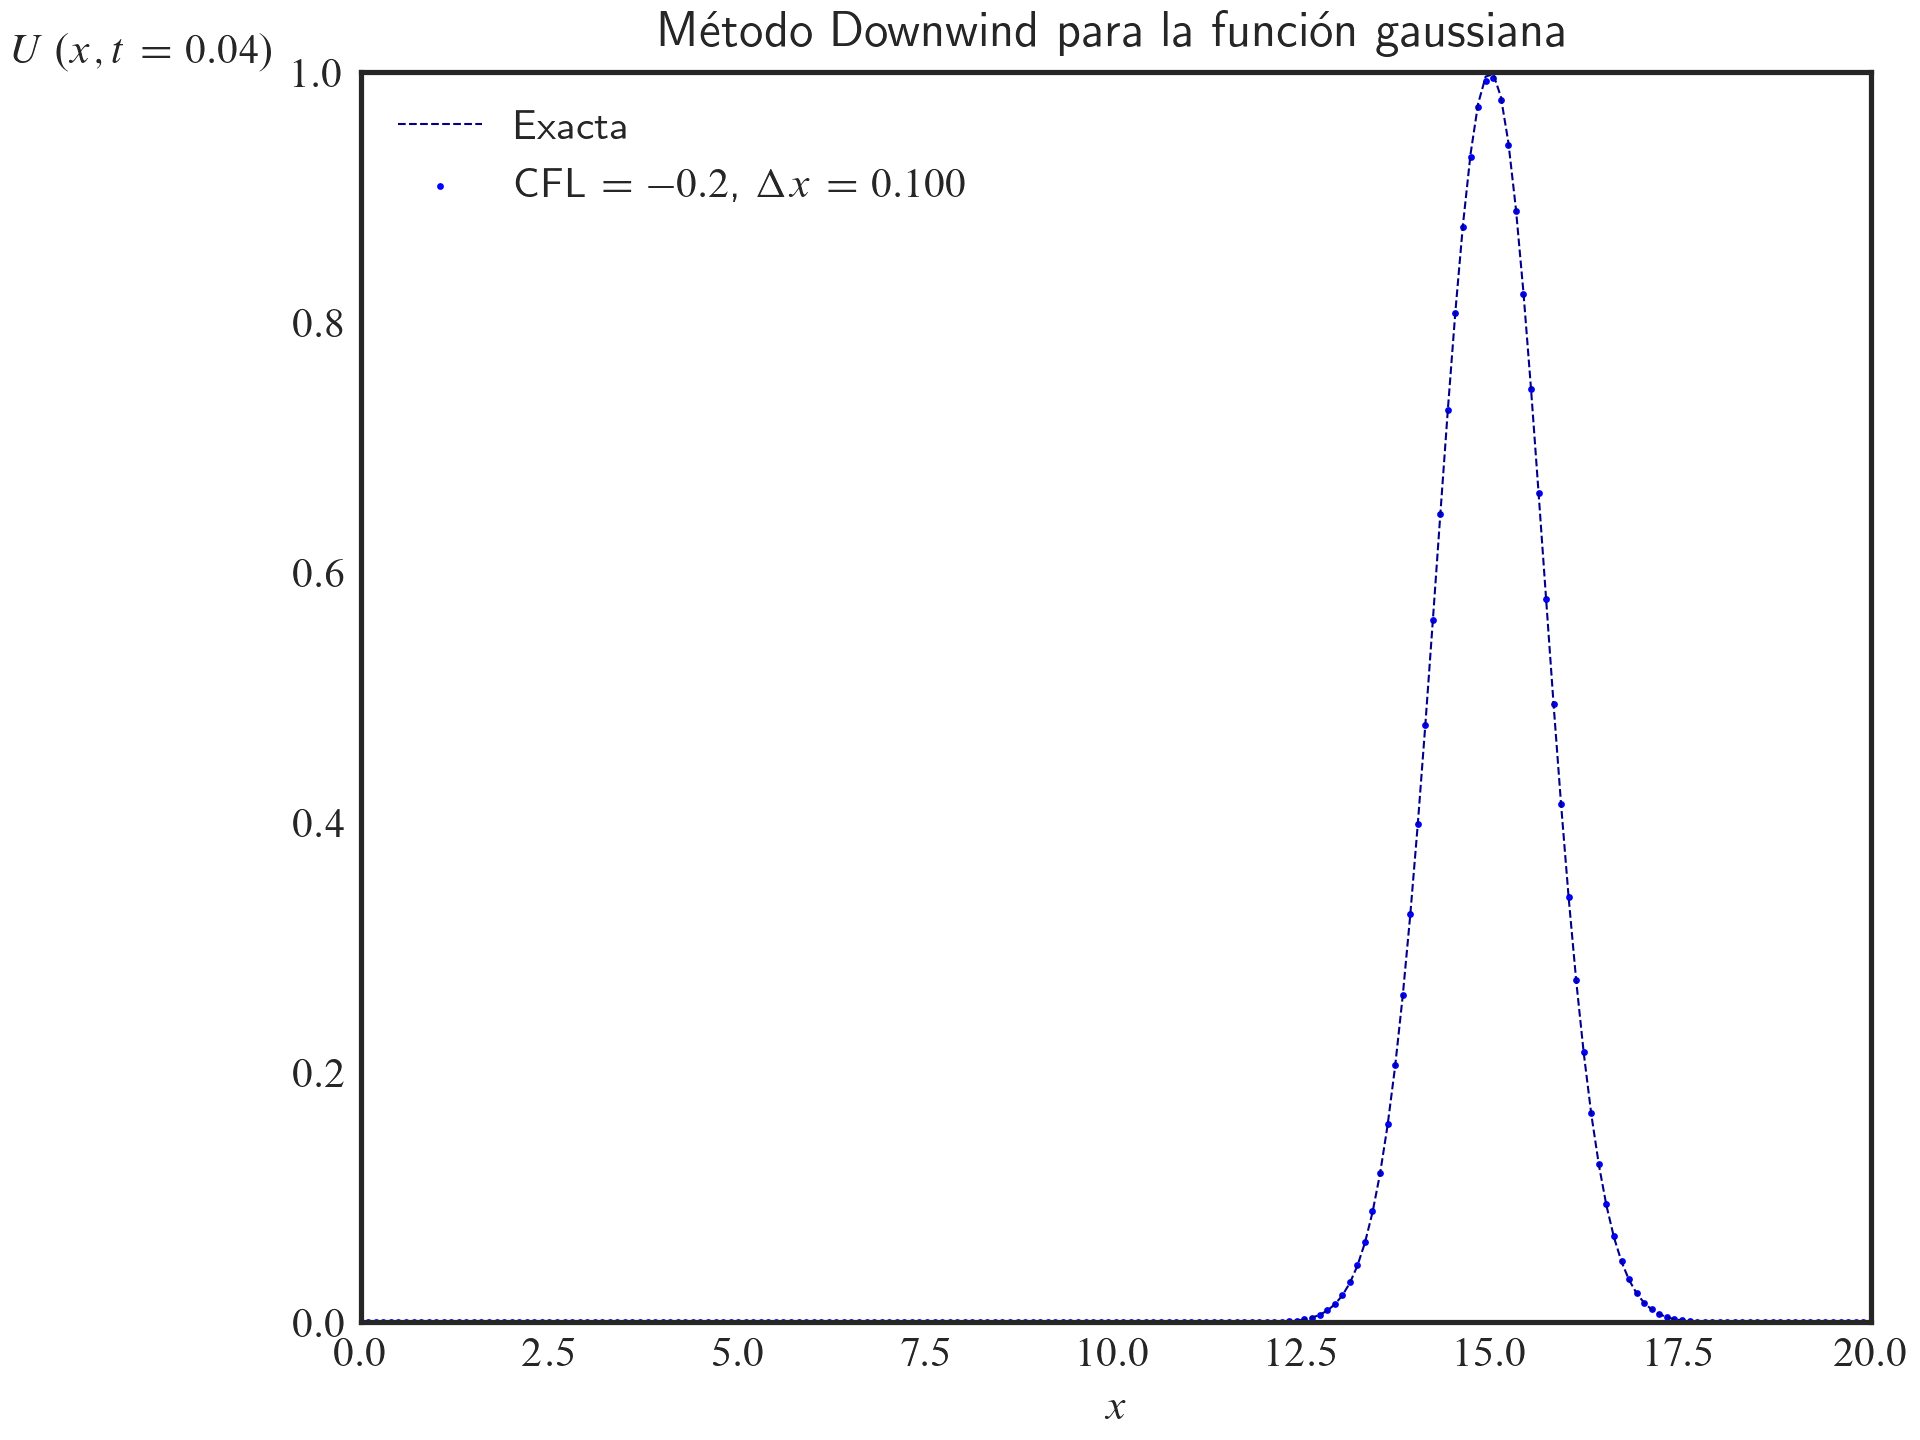
\includegraphics[width=.30\paperwidth]{../snapshots/downwindgaussian1d-2.png}
        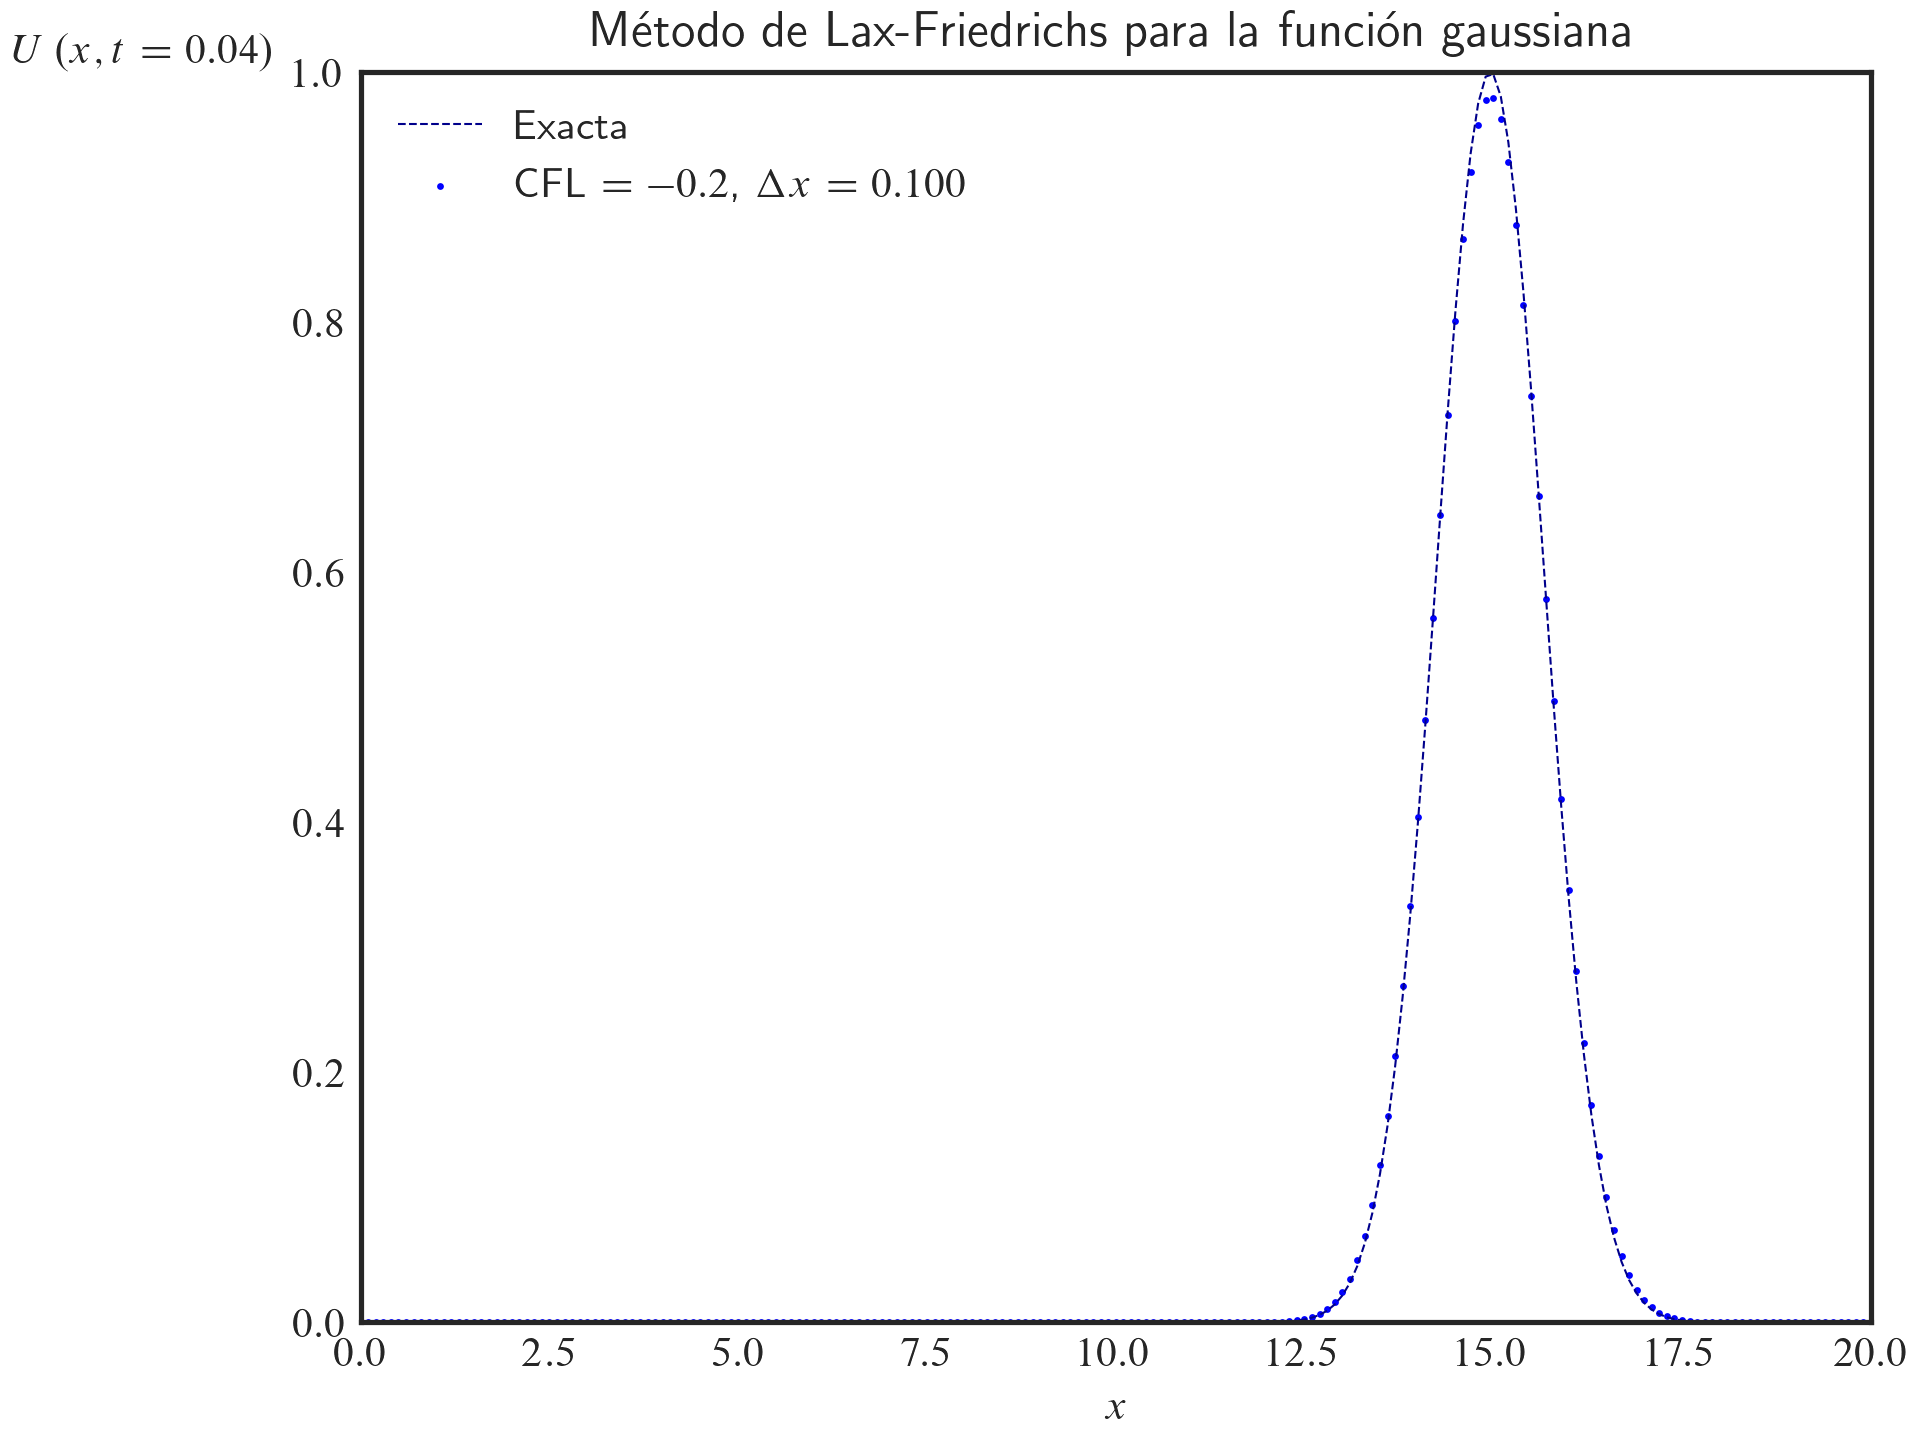
\includegraphics[width=.30\paperwidth]{../snapshots/lax-friedrichsgaussiana1d-2.png}
        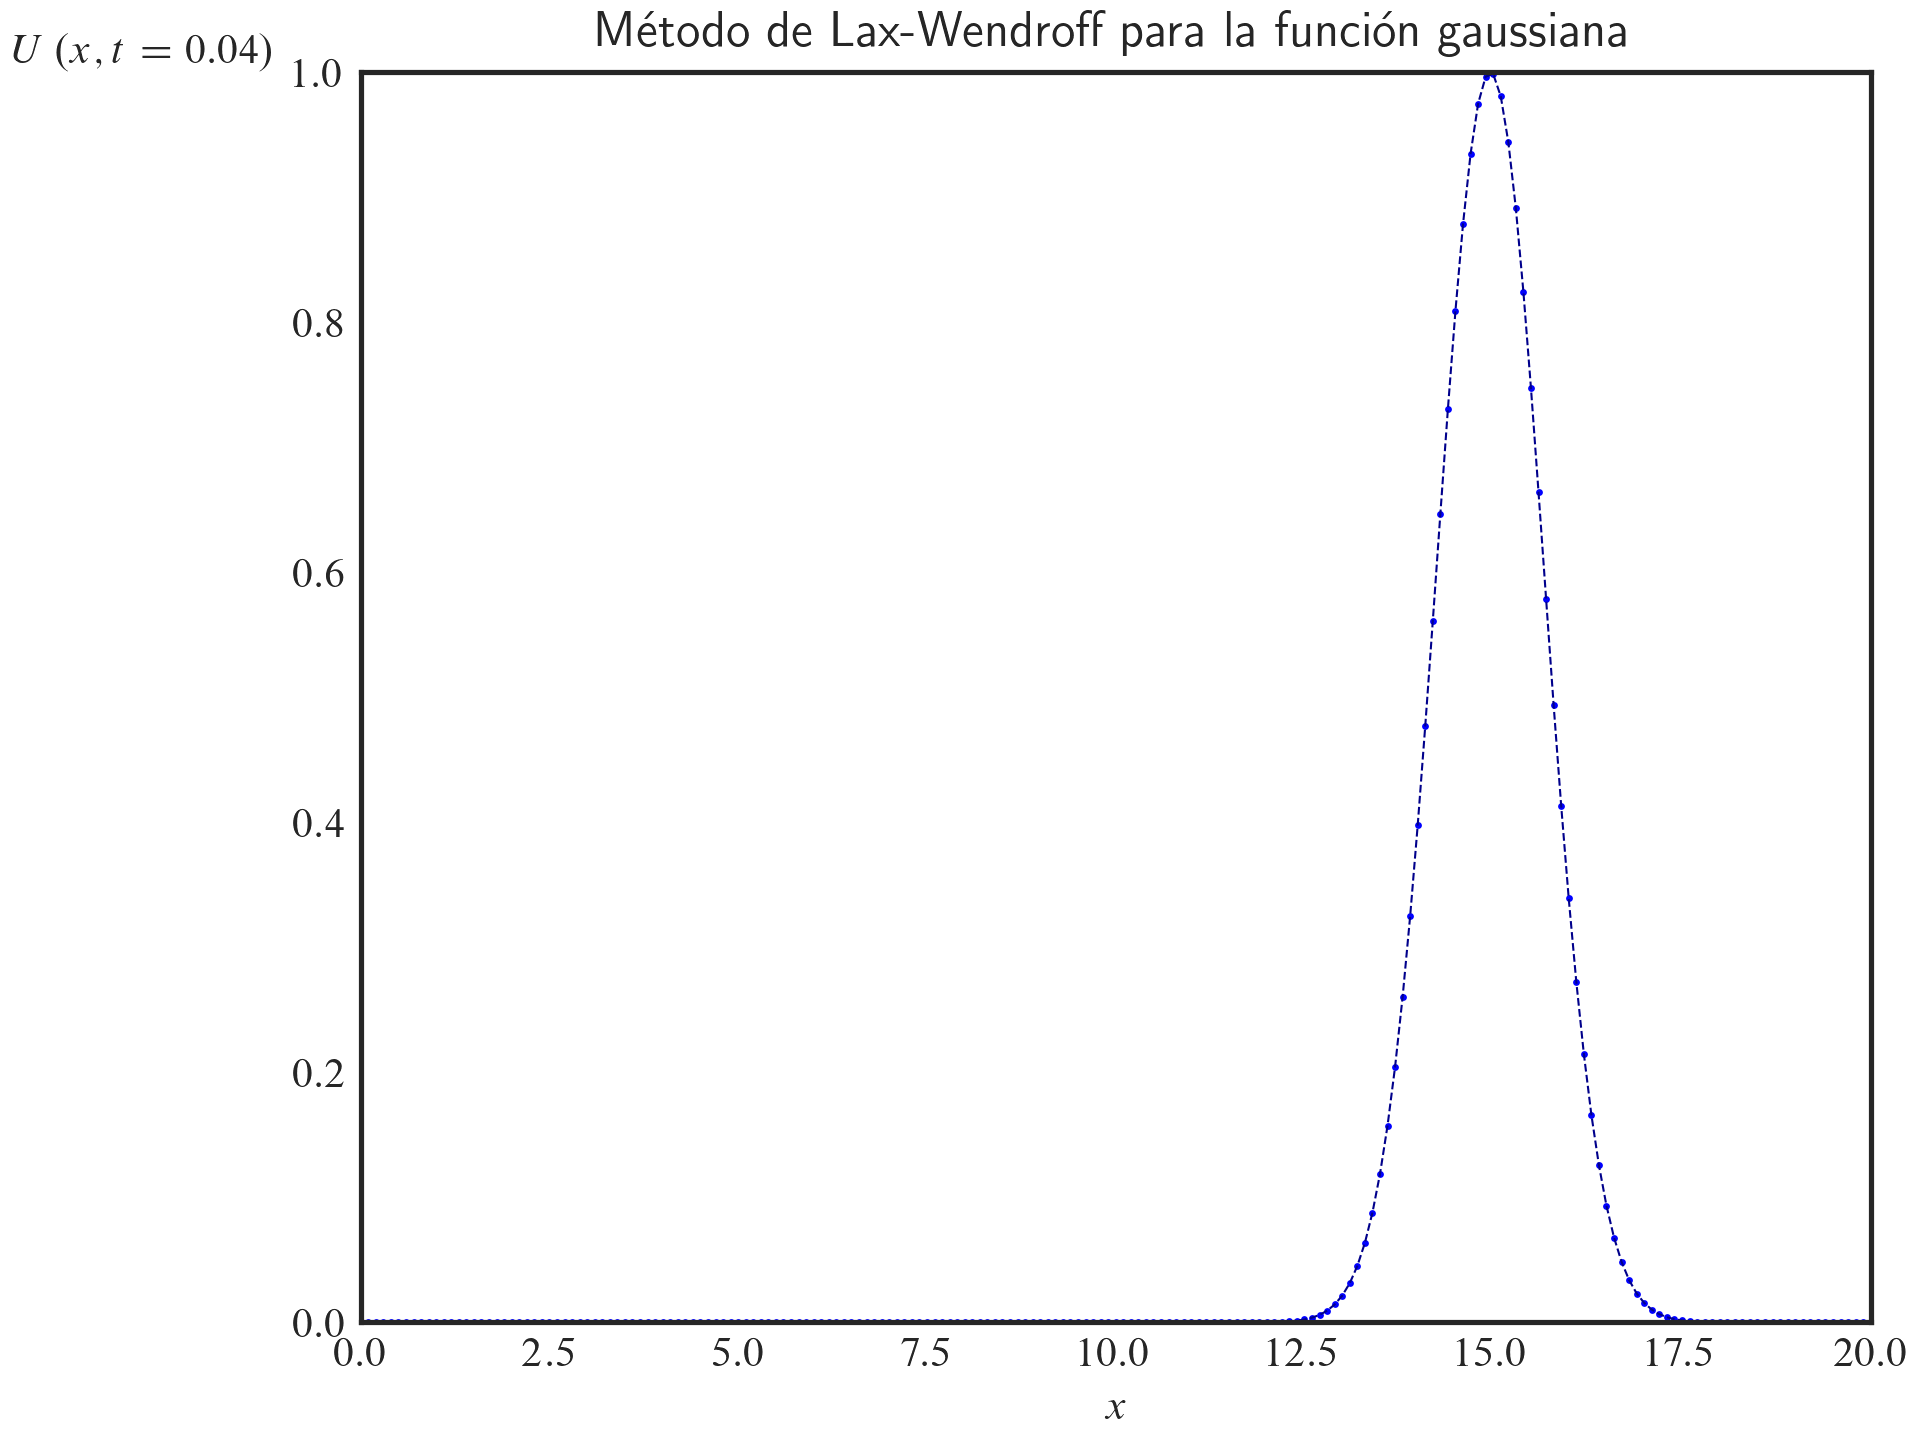
\includegraphics[width=.30\paperwidth]{../snapshots/lax-wendroffgaussiana1d-2.png}
        \caption{Simulación numérica en el tiempo $t_{2}=2\Delta t$.}
        \label{fig:example1t2}
    \end{figure}
\end{frame}

\begin{frame}
    \frametitle{\secname}

    \begin{figure}[ht!]
        \centering
        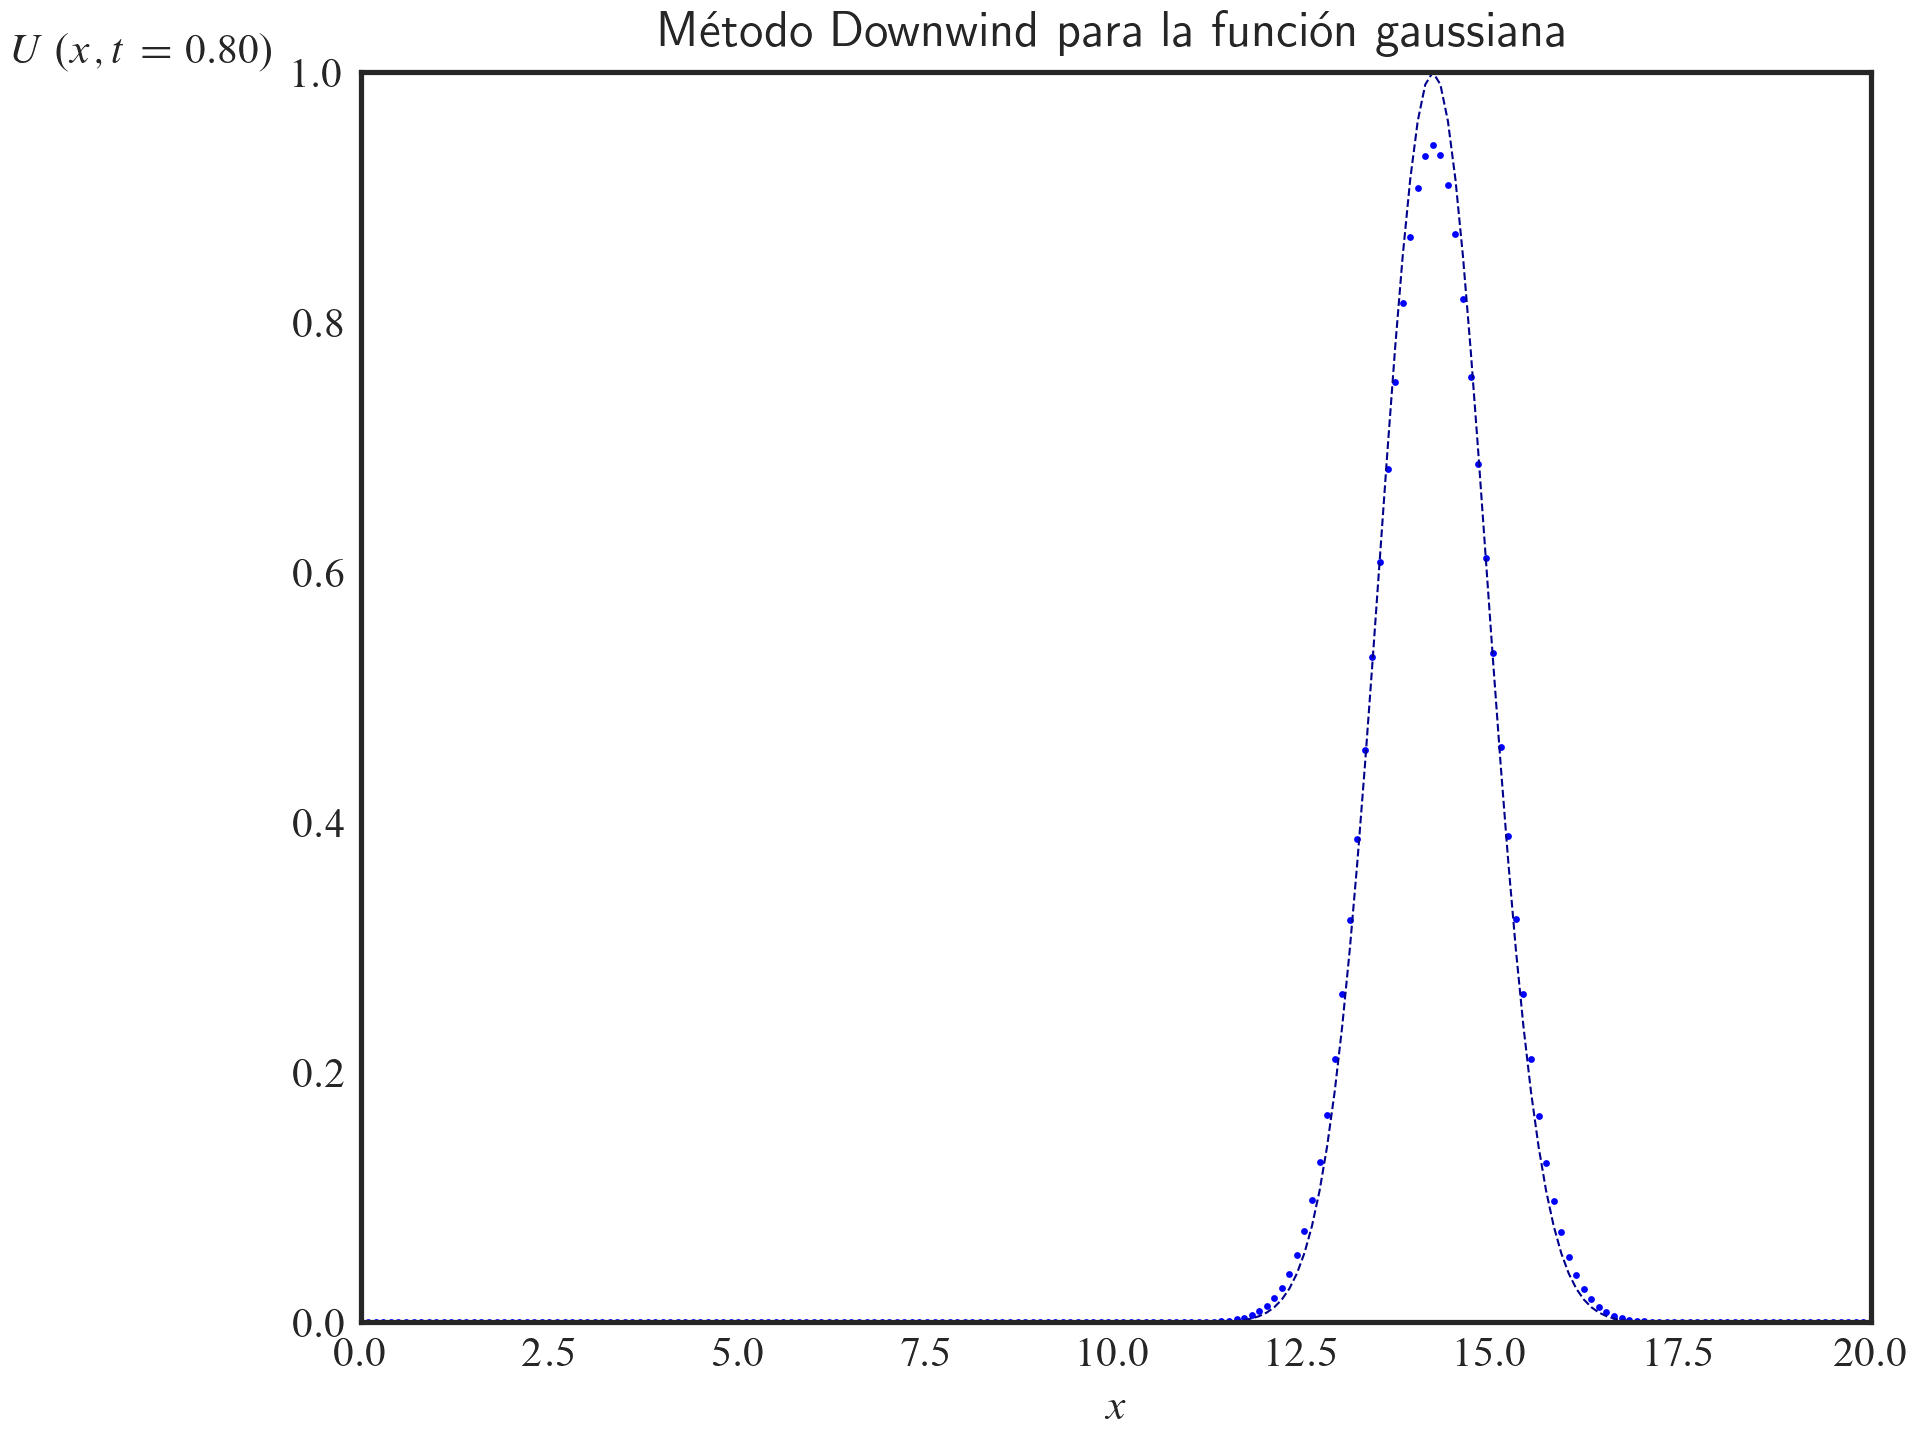
\includegraphics[width=.30\paperwidth]{../snapshots/downwindgaussian1d-40.png}
        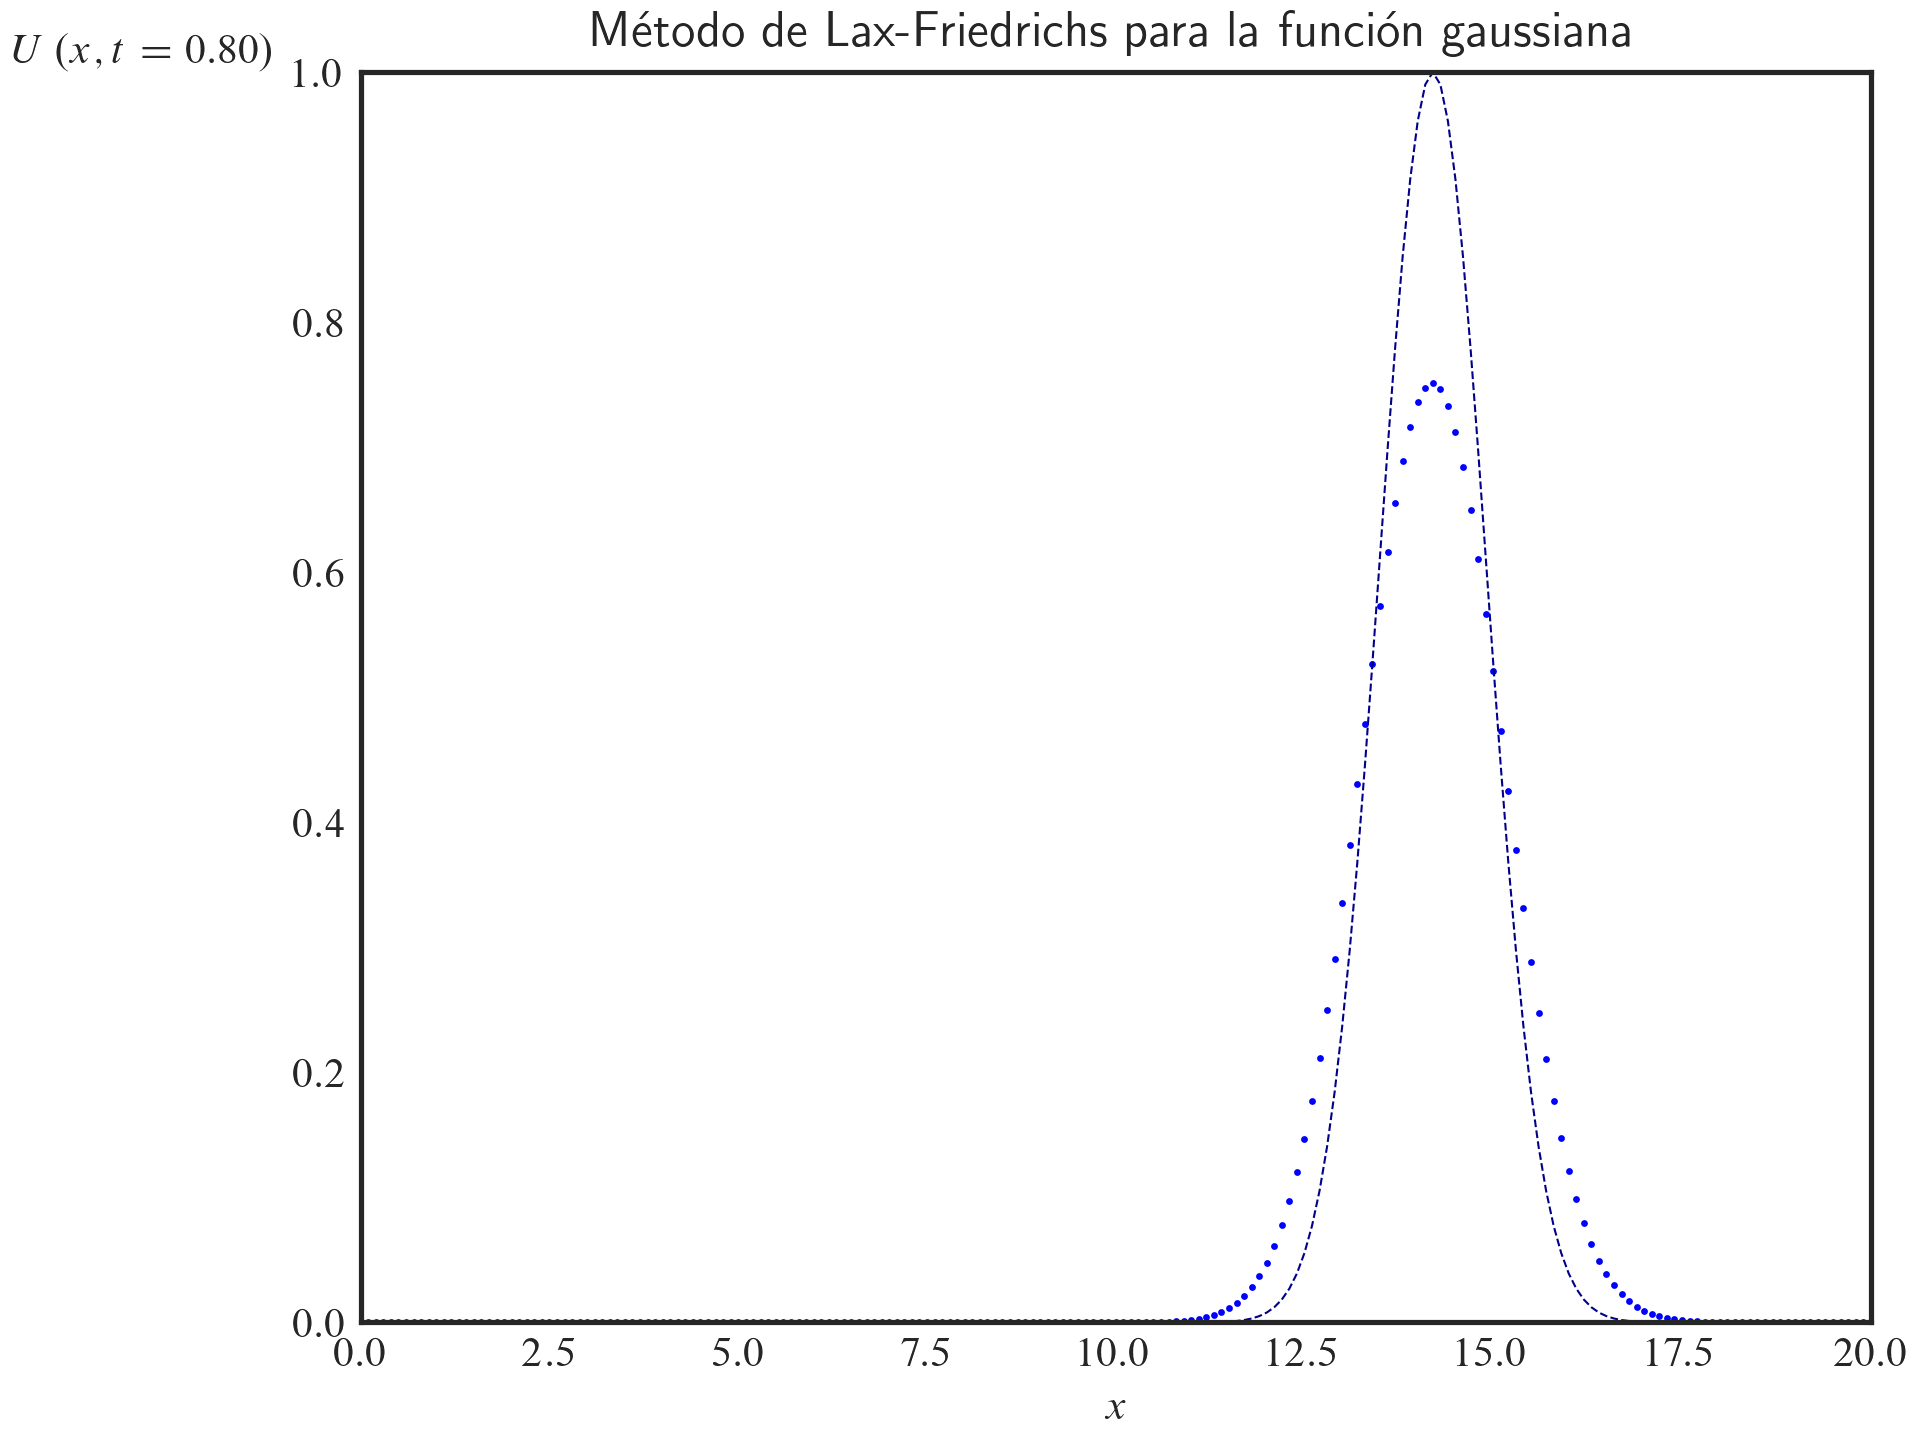
\includegraphics[width=.30\paperwidth]{../snapshots/lax-friedrichsgaussiana1d-40.png}
        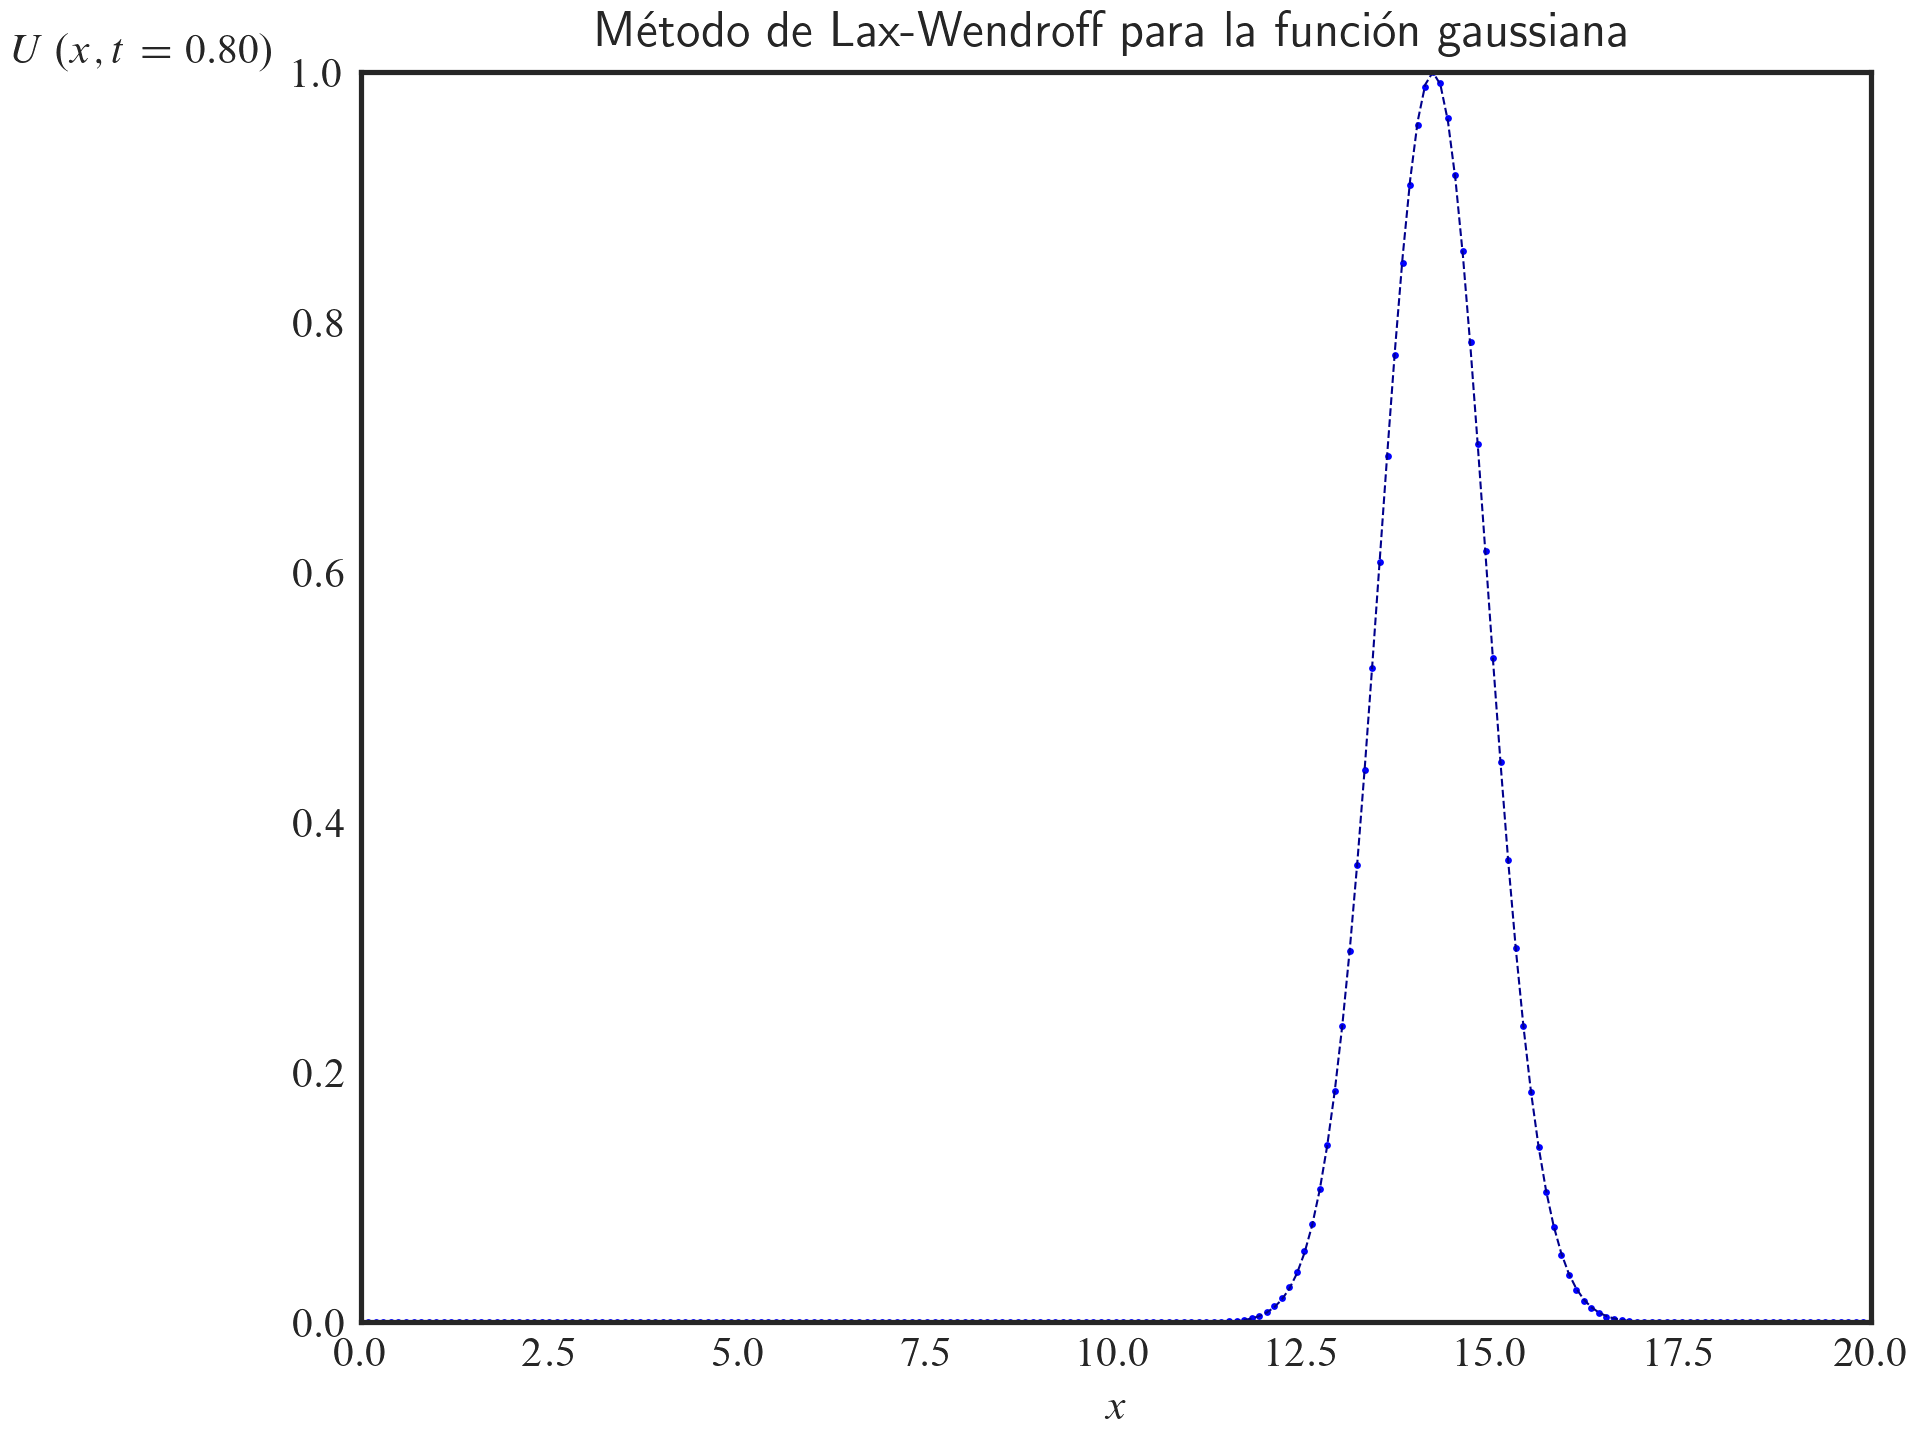
\includegraphics[width=.30\paperwidth]{../snapshots/lax-wendroffgaussiana1d-40.png}
        \caption{Simulación numérica en el tiempo $t_{40}=40\Delta t$.}
        \label{fig:example1t40}
    \end{figure}
\end{frame}

\begin{frame}
    \frametitle{\secname}
    \begin{example}
        En este ejemplo consideramos el dominio espacial
        $\Omega=\left[0,30\right]$, el paso en espacio $\Delta x=0.12$, el
        paso en tiempo $\Delta t=0.02$, la velocidad de propagación positiva
        $c=1$ (para los que se verifica la condición CFL) y la condición
        inicial dada por la función discontinua

        \begin{equation*}
            u_{0}\left(x\right)=
            \begin{cases}
                2, & \text{si }x<15, \\
                1, & \text{si }x>15.
            \end{cases}
        \end{equation*}

        Para este dato inicial calculamos las soluciones numéricas de la
        ecuación de transporte~\eqref{eq:transportequation}, aplicando el
        método descentrado upwind, el método de Lax-Friedrichs y por último,
        el método de Lax-Wendroff.
        Al igual que en el ejemplo anterior, hemos empleado el lenguaje de
        programación Python.
        Entonces, obtenemos los resultados de las
        Figuras~\ref{fig:example2t2} y~\ref{fig:example2t10} (donde se
        reproduce el mismo experimento pero en los instantes de tiempo
        $t_{2}=0.04$ y $t_{10}=0.2$), para cada uno de los métodos nombrados
        junto con la solución exacta y para cada instante de tiempo
        considerado.
    \end{example}
\end{frame}

\begin{frame}
    \frametitle{\secname}

    \begin{figure}[ht!]
        \centering
        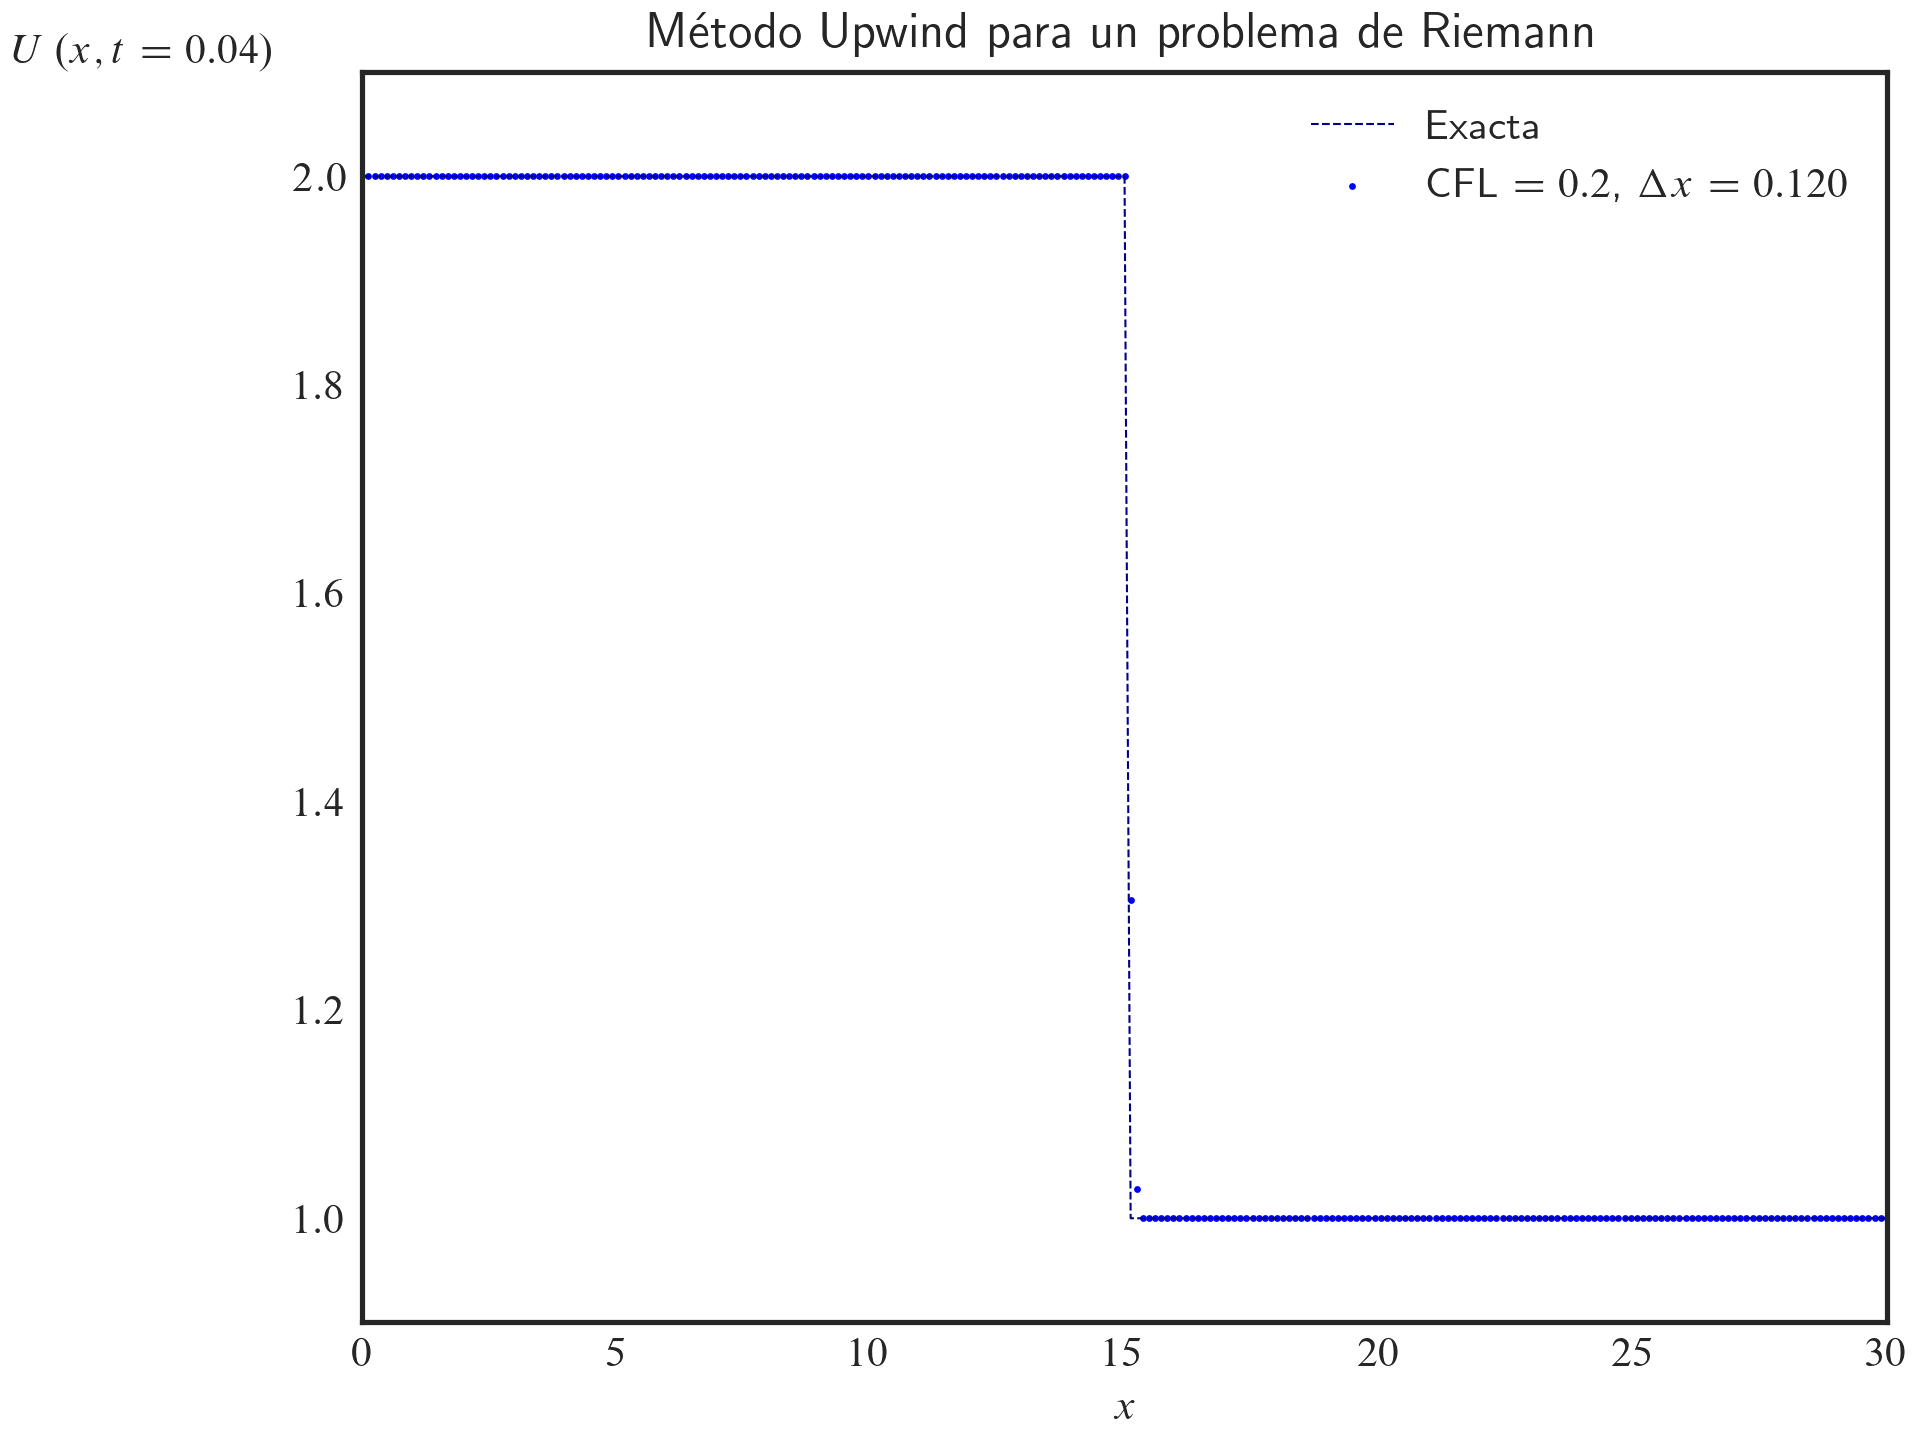
\includegraphics[width=.30\paperwidth]{../snapshots/upwindheaviside1d-2.png}
        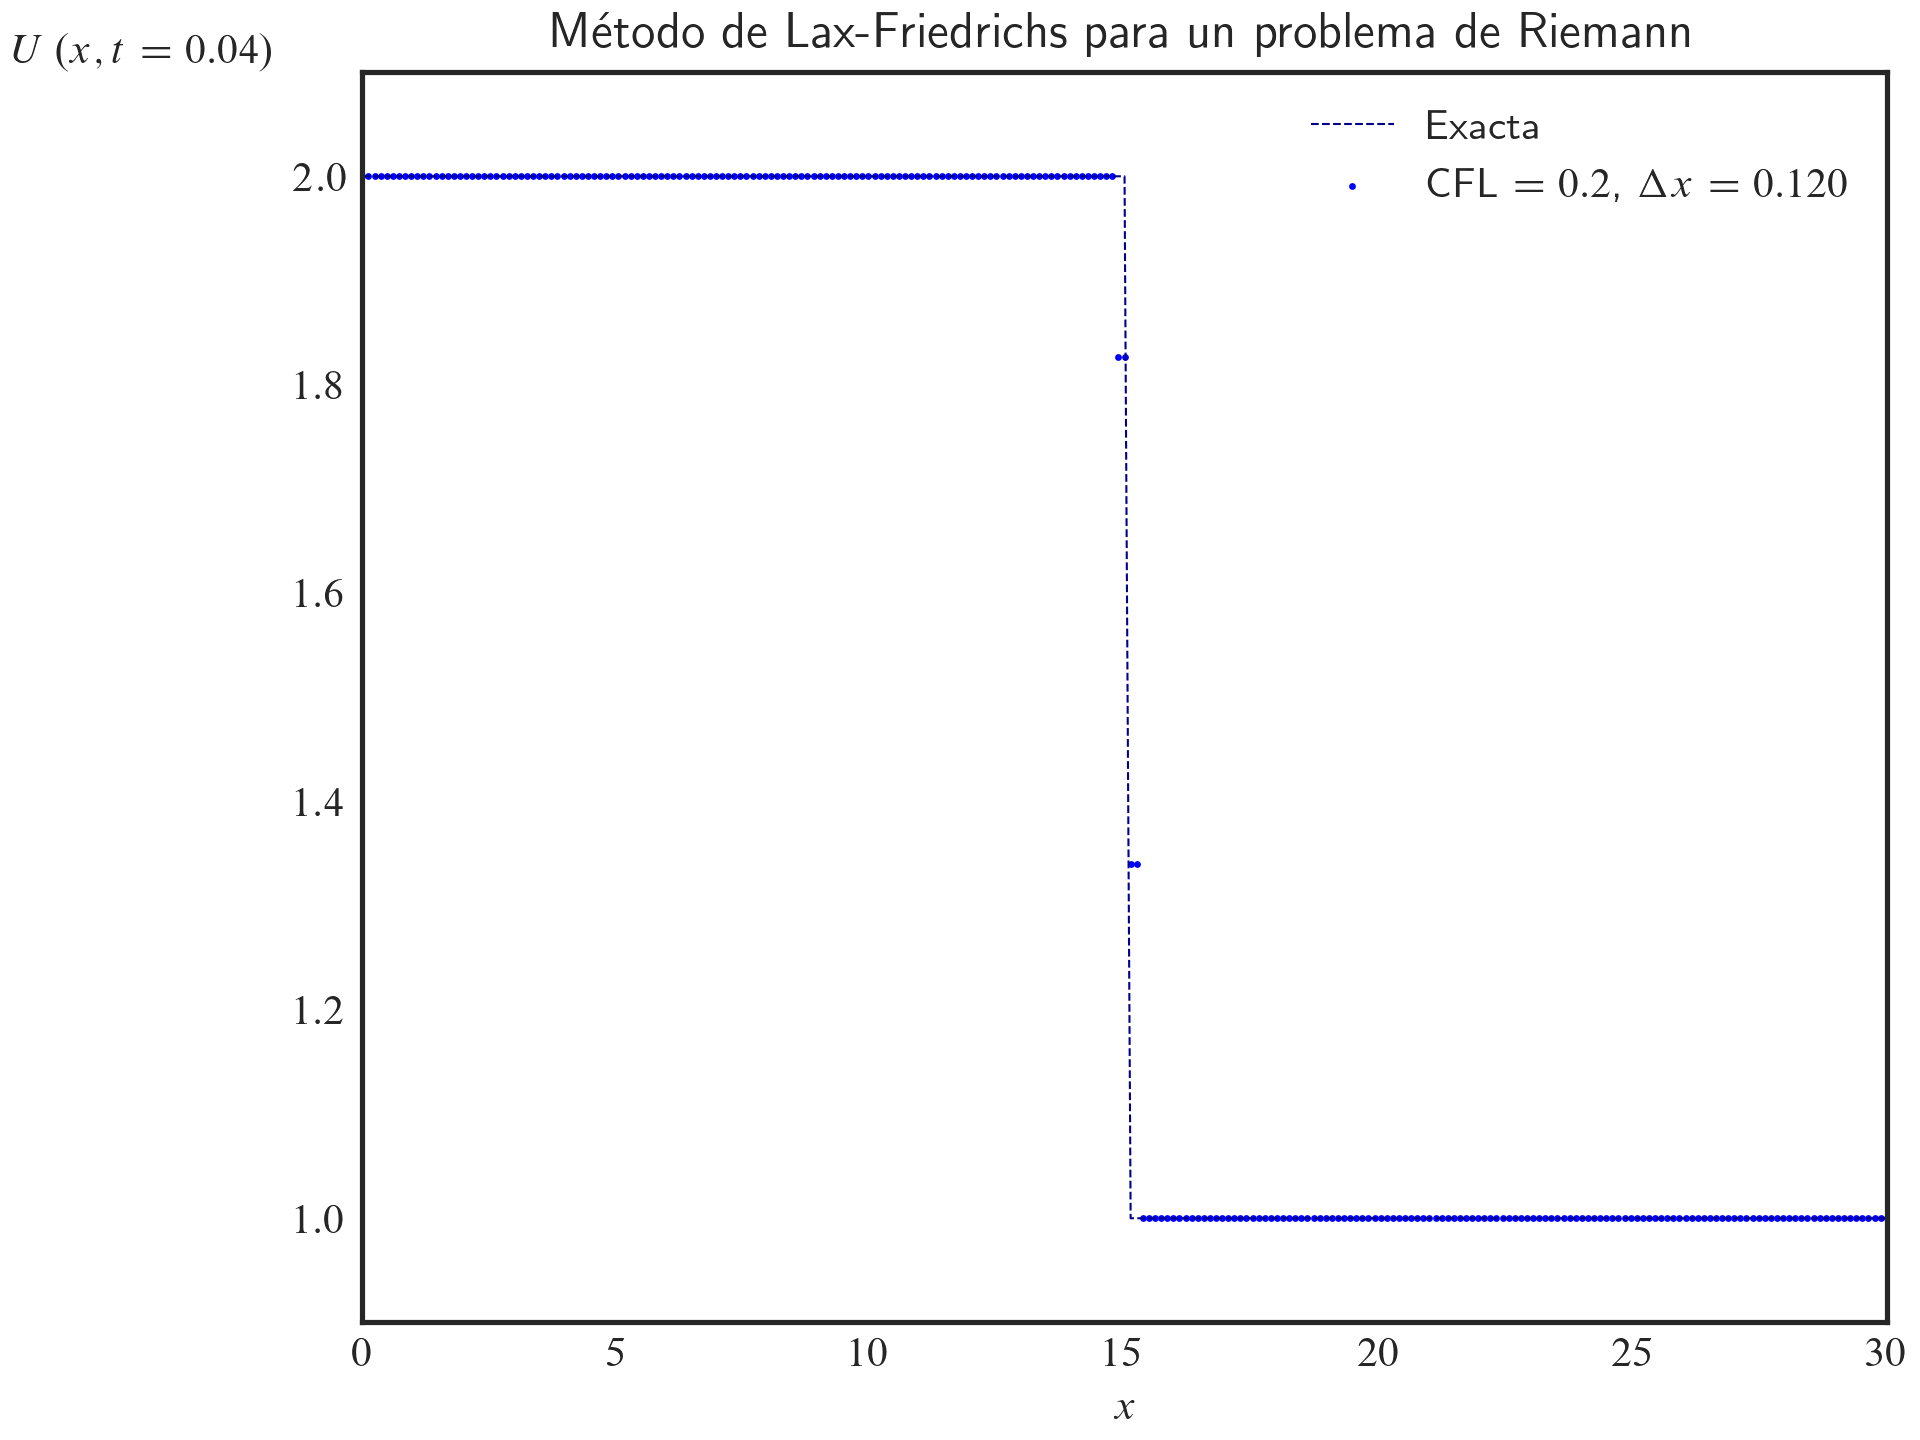
\includegraphics[width=.30\paperwidth]{../snapshots/lax-friedrichsheaviside1d-2.png}
        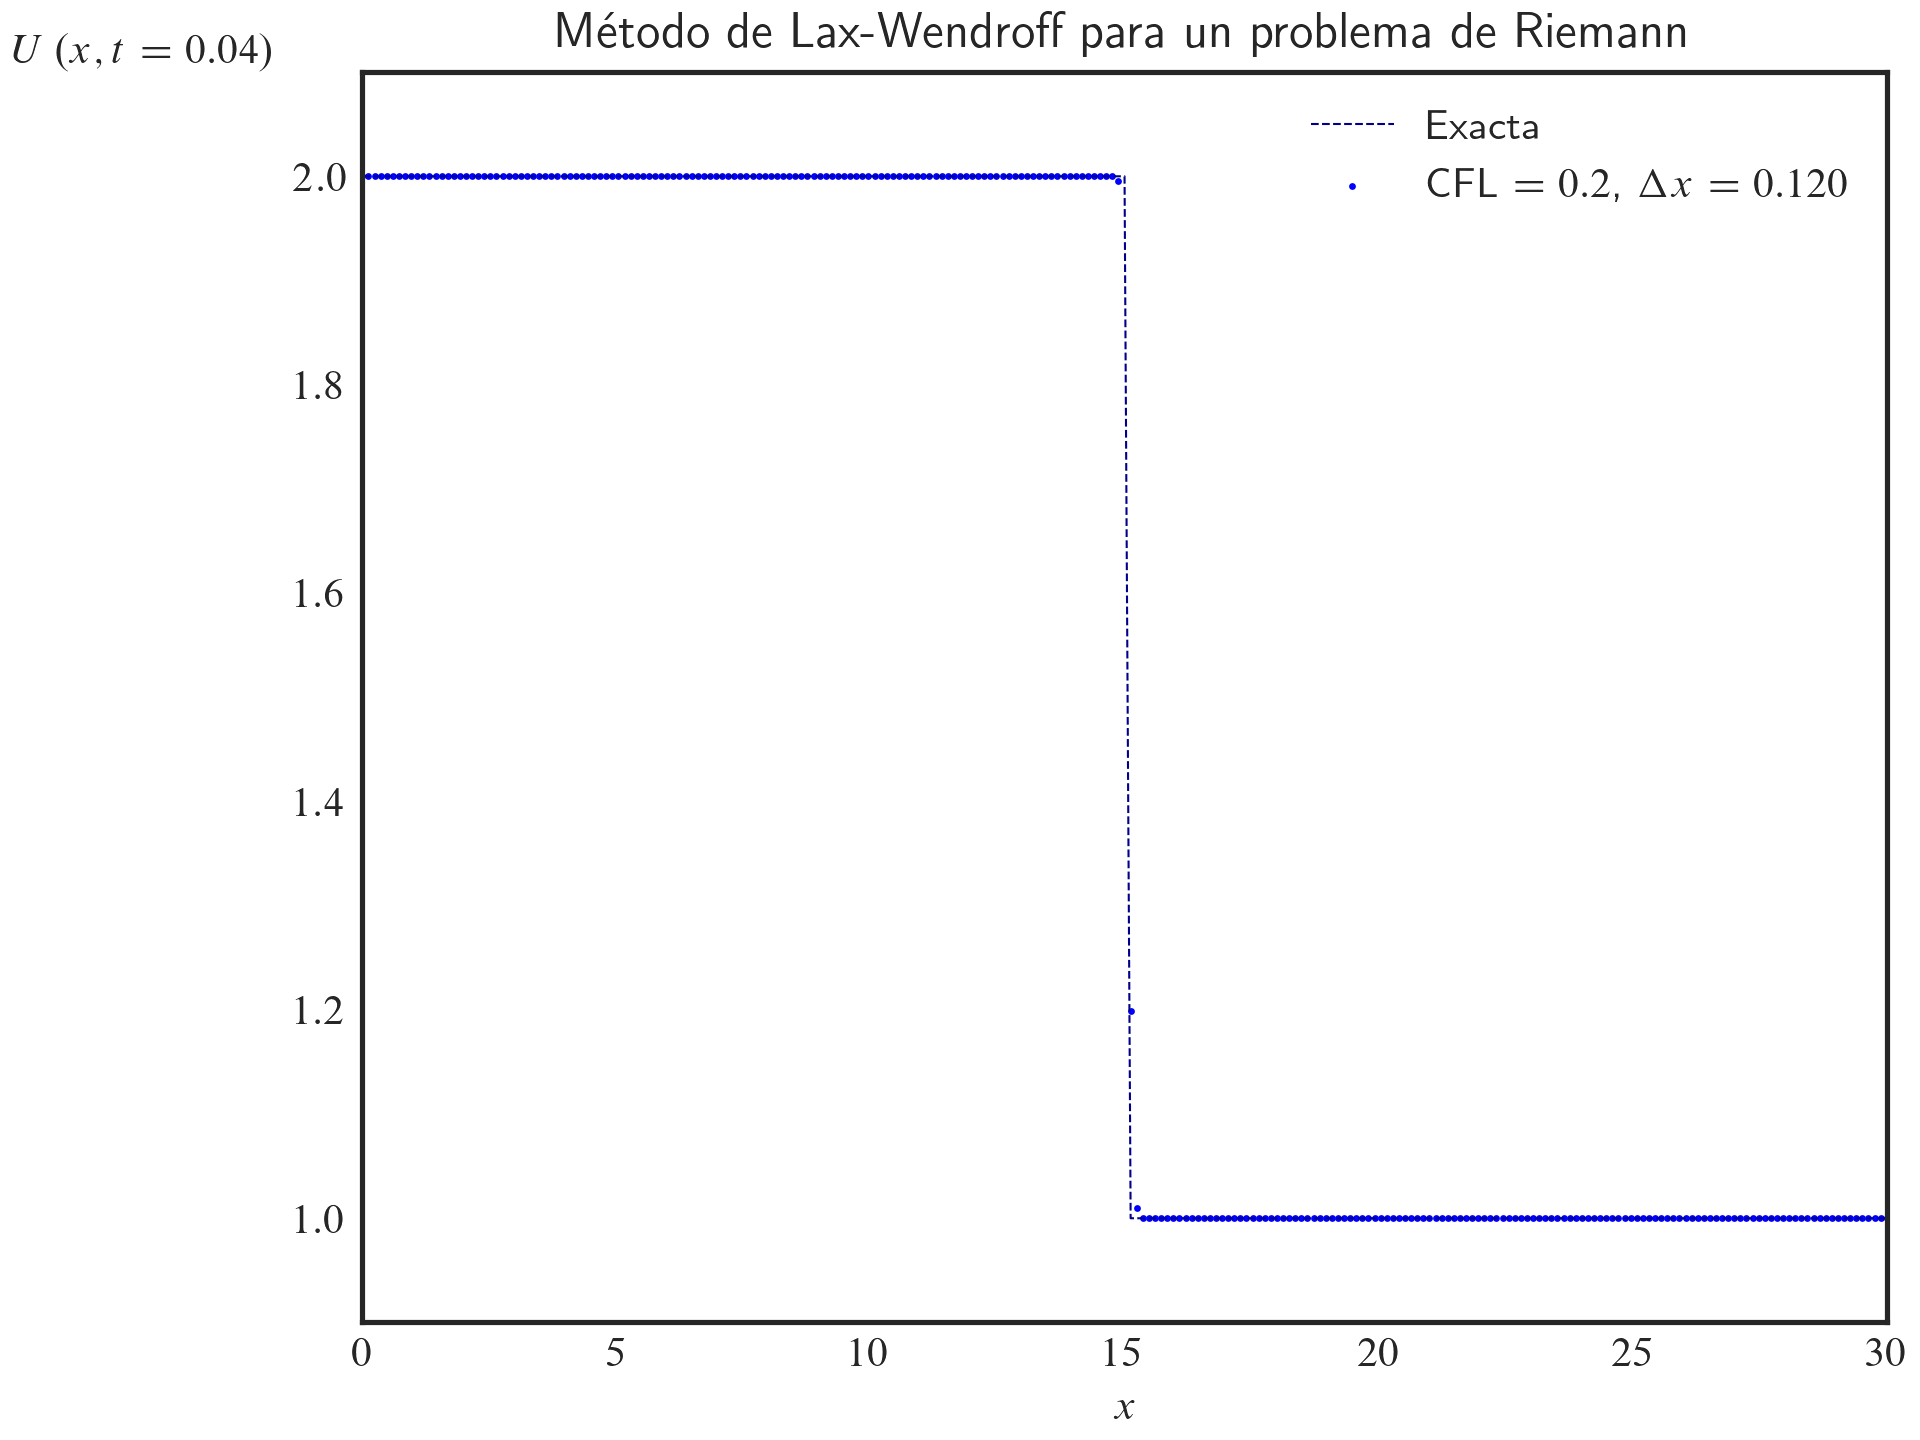
\includegraphics[width=.30\paperwidth]{../snapshots/lax-wendroffheaviside1d-2.png}
        \caption{Simulación numérica en el tiempo $t_{2}=2\Delta t$.}
        \label{fig:example2t2}
    \end{figure}

\end{frame}

\begin{frame}
    \frametitle{\secname}

    \begin{figure}[ht!]
        \centering
        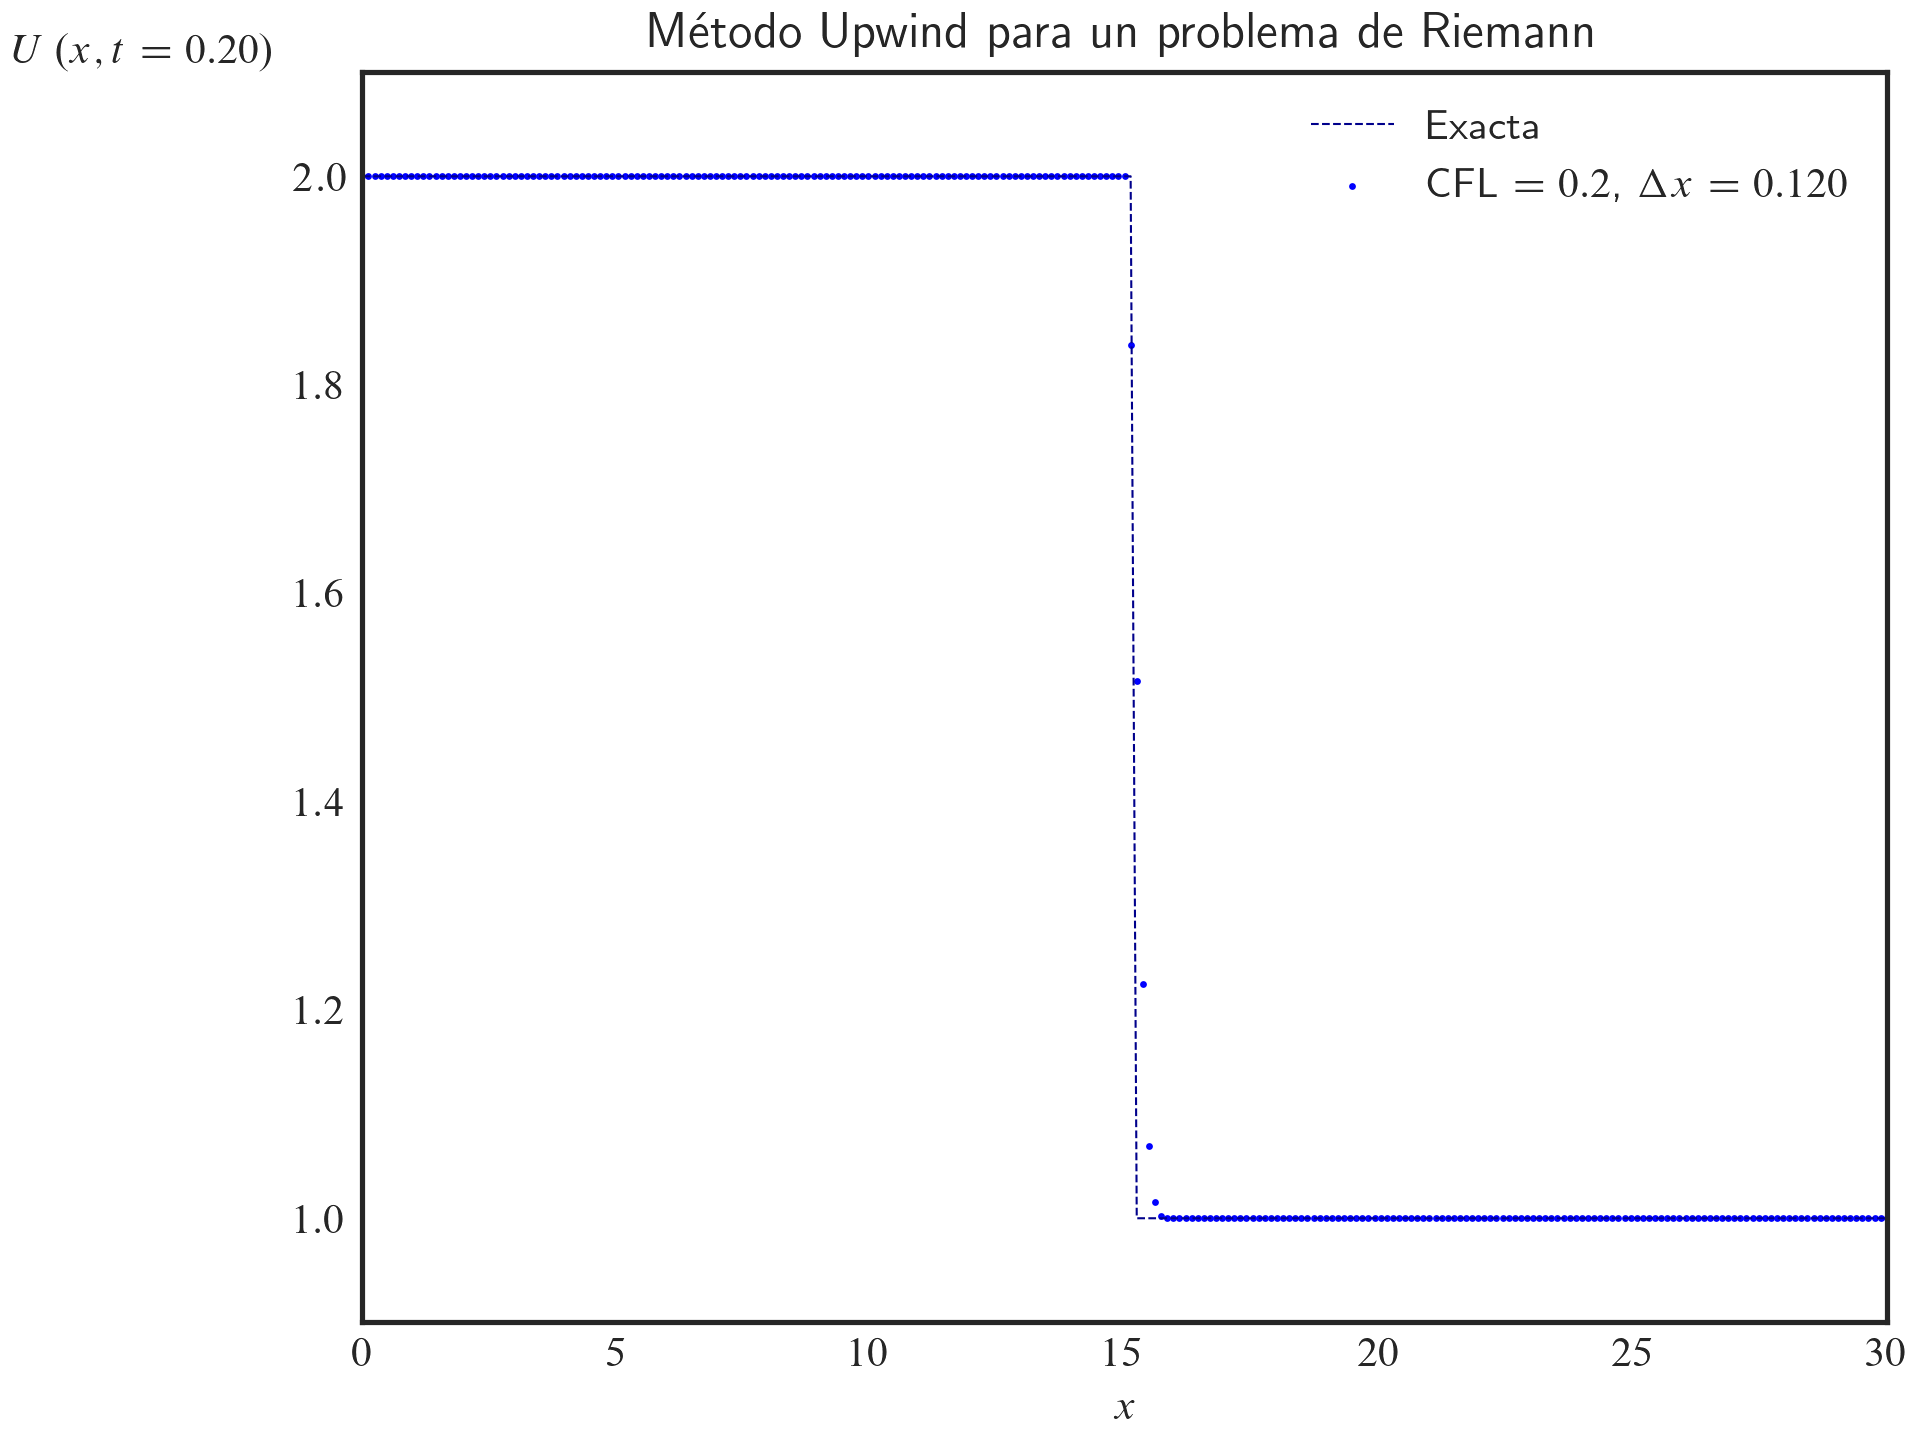
\includegraphics[width=.30\paperwidth]{../snapshots/upwindheaviside1d-10.png}
        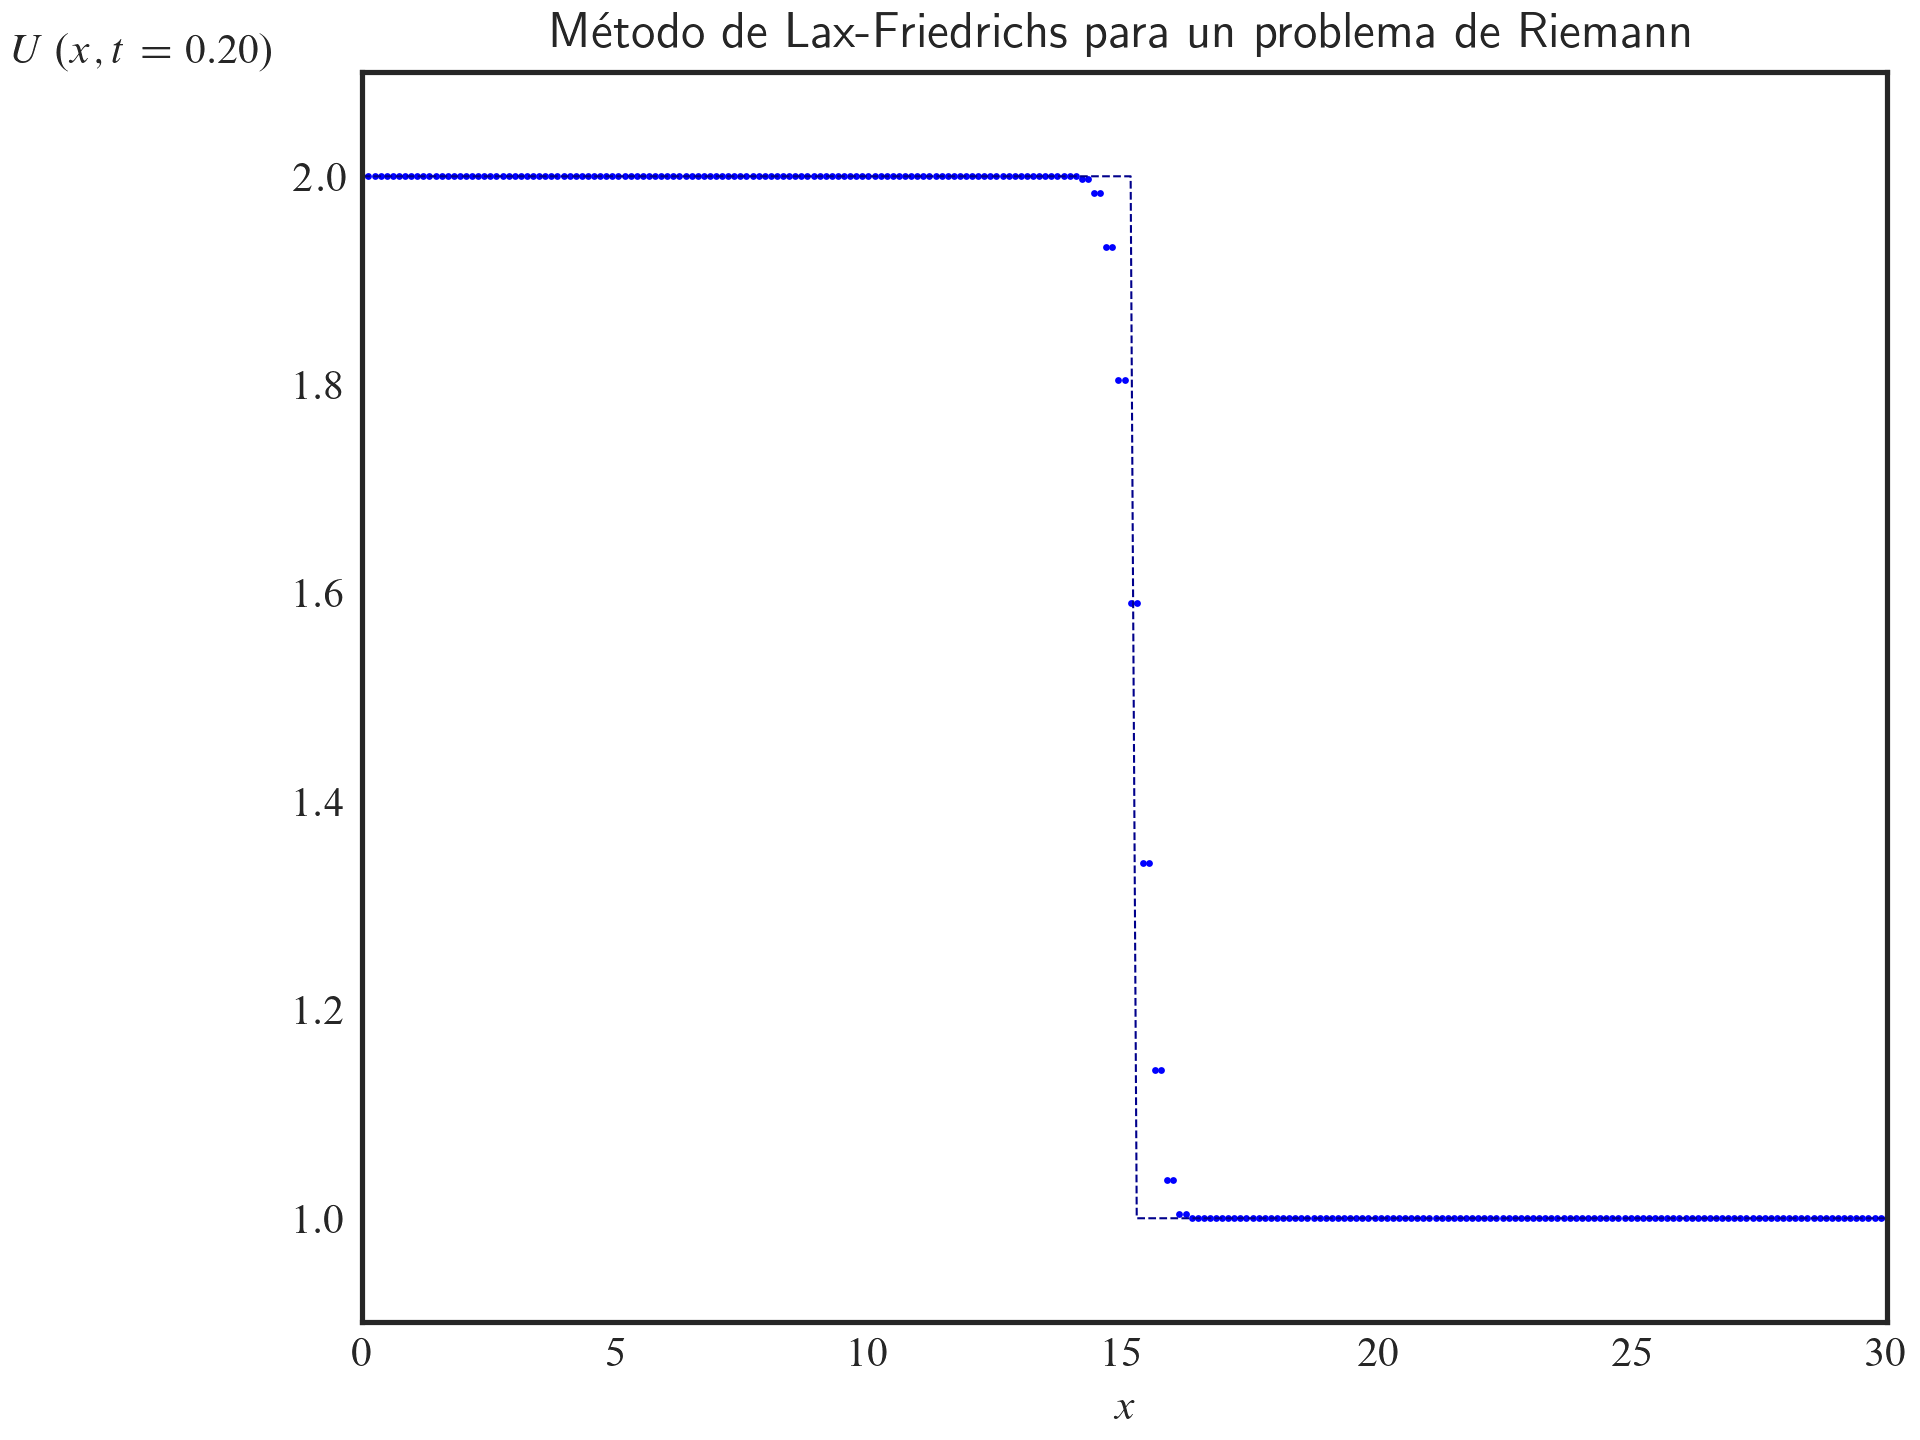
\includegraphics[width=.30\paperwidth]{../snapshots/lax-friedrichsheaviside1d-10.png}
        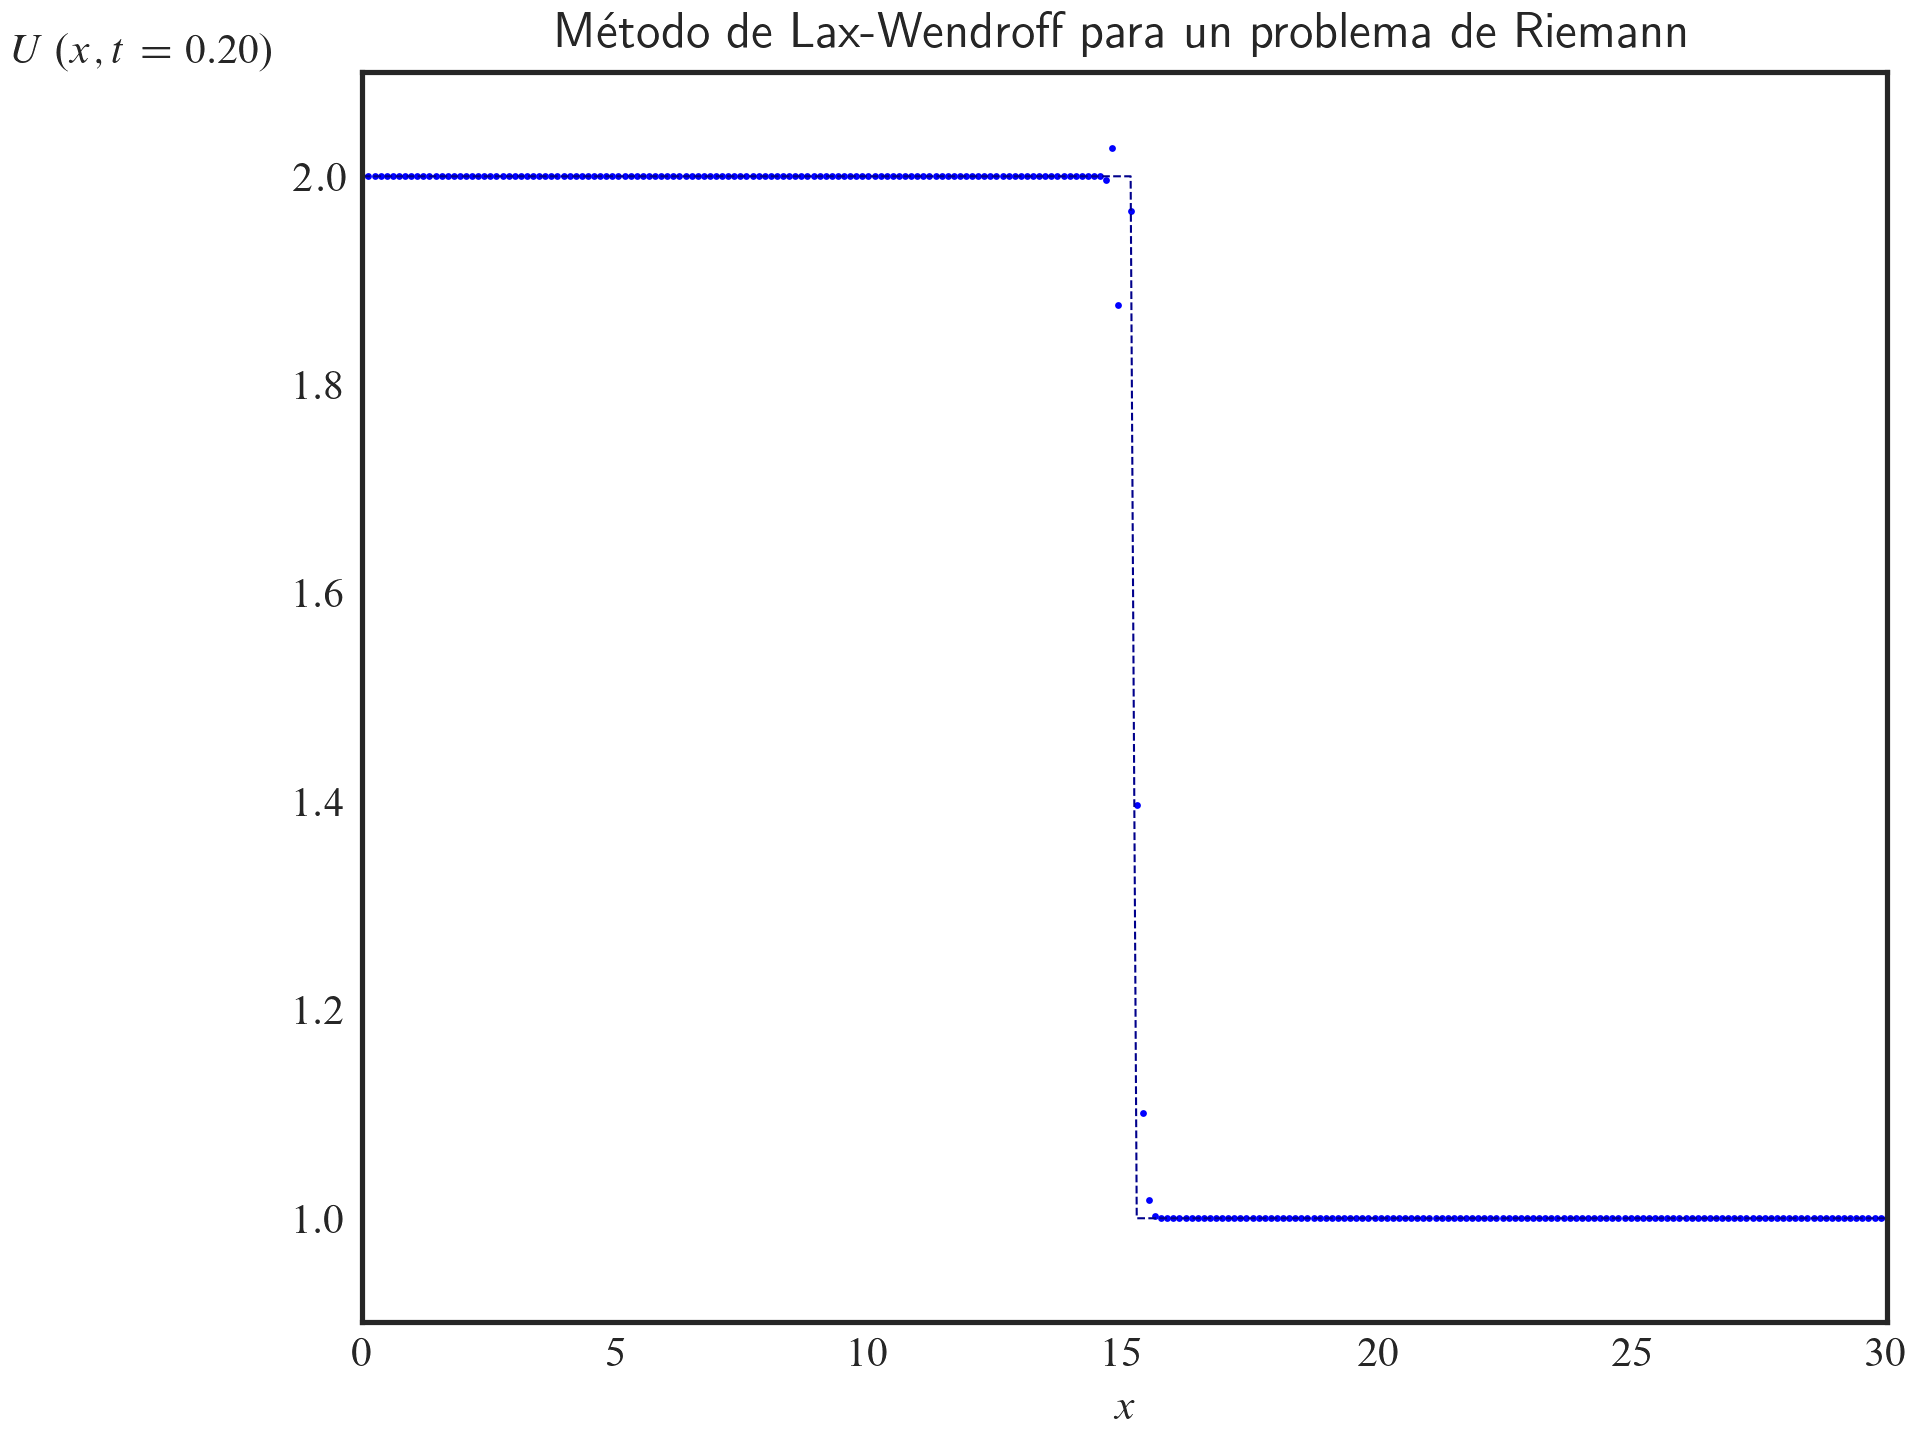
\includegraphics[width=.30\paperwidth]{../snapshots/lax-wendroffheaviside1d-10.png}
        \caption{Simulación numérica en el tiempo $t_{10}=10\Delta t$.}
        \label{fig:example2t10}
    \end{figure}
\end{frame}
\section{Conclusiones y algunas preguntas abiertas}

\begin{frame}
	\frametitle{Conclusiones}

	\begin{itemize}
		\item Se ha superado el problema de las oscilaciones espurias.
	\end{itemize}
\end{frame}


\backmatter

\appendix

\chapter{Condición de salto Rankine-Hugoniot}

\begin{theorem}
  El salto $u_{r}-u_{l}$, a través de la discontinuidad, es un
  múltiplo escalar del autovector asociado al autovalor $\lambda$ de
  la ecuación $u_{t}+\lambda u_{x}=0$.
\end{theorem}

\begin{proof}
  Sabemos que $\lambda$ es la velocidad con la que se propaga esta
  discontinuidad, asumimos que es negativa.
  Estudiémosla en el rectángulo de espacio y tiempo
  \begin{math}
    \left[x_{1},x_{1}+\Delta x\right]\times
    \left[t_{1},t_{1}+\Delta t\right]
  \end{math}.
  Como se muestra en la Figura~\ref{fig:2}

  \begin{figure}[ht!]
    \centering
    \includegraphics[width=.4\paperwidth]{figure2}
    \caption{Región infinitesimal rectangular en el plano $xt$.}
    \label{fig:2}
  \end{figure}

  Aplicamos la forma integral de la ley de
  conservación~\eqref{eq:integralconservationlaw} a esta región,
  entonces obtenemos

  \begin{equation*}
    \diffp{}{t}
    \int_{x_{1}}^{x_{1}+\Delta x}
    u\left(x,t\right)\dl x=
    f\left(u\left(x_{1},t\right)\right)-
    f\left(u\left(x_{1}+\Delta x,t\right)\right).
  \end{equation*}

  Integrando en tiempo en el intervalo
  $\left[t_{1},t_{1}+\Delta t\right]$ tenemos
  \begin{equation*}
    \int_{x_{1}}^{x_{1}+\Delta x}
    u\left(x,t_{1}+\Delta t\right)-
    \int_{x_{1}}^{x_{1}+\Delta x}
    u\left(x,t_{1}\right)=
    \int_{t_{1}}^{t_{1}+\Delta t}
    f\left(u\left(x_{1},t\right)\right)
    \dl t-
    \int_{t_{1}}^{t_{1}+\Delta t}
    f\left(u\left(x_{1}+\Delta x,t\right)\right)
    \dl t
  \end{equation*}

  Entonces, como la función flujo es lineal y $u$ es constante en
  cada porción del plano,

  \begin{equation}\label{eq:difference}
    \Delta x u_{r}-
    \Delta x u_{l}=
    \Delta t f\left(u_{l}\right)-
    \Delta t f\left(u_{r}\right).
  \end{equation}

  Dado que $\lambda$ es la velocidad de propagación, negativa,
  entonces $\Delta x=-\lambda\Delta t$.
  Dividiendo la igualdad~\eqref{eq:difference} entre $-\Delta t$, y
  como $\Delta x=-\lambda\Delta t$, obtenemos

  \begin{equation*}
    \lambda\left(u_{r}-u_{l}\right)=
    f\left(u_{r}\right)-
    f\left(u_{l}\right),
  \end{equation*}

  y por lo tanto el salto $u_{r}-u_{l}$ es múltiplo del autovector
  asociado a $\lambda$ como queríamos ver.
  Esta ecuación se denomina condición de salto de Rankine-Hugoniot.
\end{proof}
\chapter{Códigos empleados}

\end{document}